\section*{Anhang}

\begin{figure}[h]
    \centering
    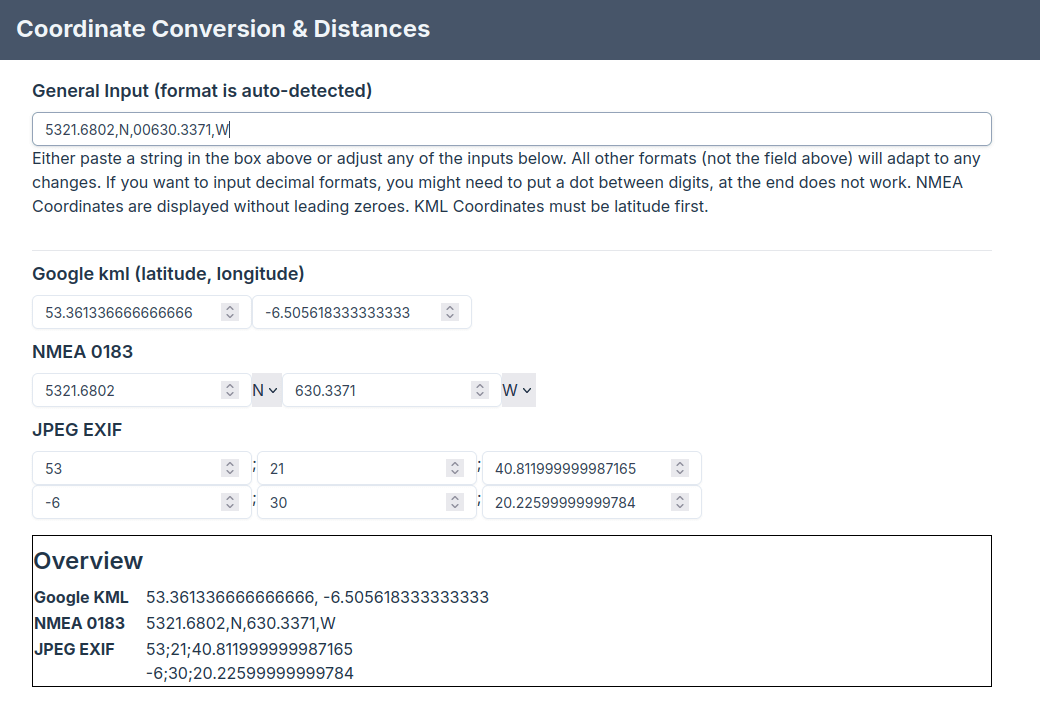
\includegraphics[width=0.9\textwidth]{figures/koordinaten.png}
    \caption{Screenshot der Webapp für die Konvertierung von Koordinatenformaten für Aufgabe \ref{sec:coord-conversion}.}
    \label{webapp-coordinates}
\end{figure}


\begin{figure}[h]
    \centering
    \includegraphics[width=0.7\textwidth]{figures/rssi_facets.pdf}
    \caption{RSSI-Messwerte der drei Apps, für Aufgabe \ref{sec:rssi}.}
    \label{rssi-facet}
\end{figure}

\begin{figure}[h]
    \centering
    \includegraphics[width=0.7\textwidth]{figures/rssi_facets_log.pdf}
    \caption{RSSI-Messwerte der drei Apps mit logarithmischer Distanz, für Aufgabe \ref{sec:rssi}.}
    \label{rssi-log}
\end{figure}


\begin{figure}[h]
    \centering
    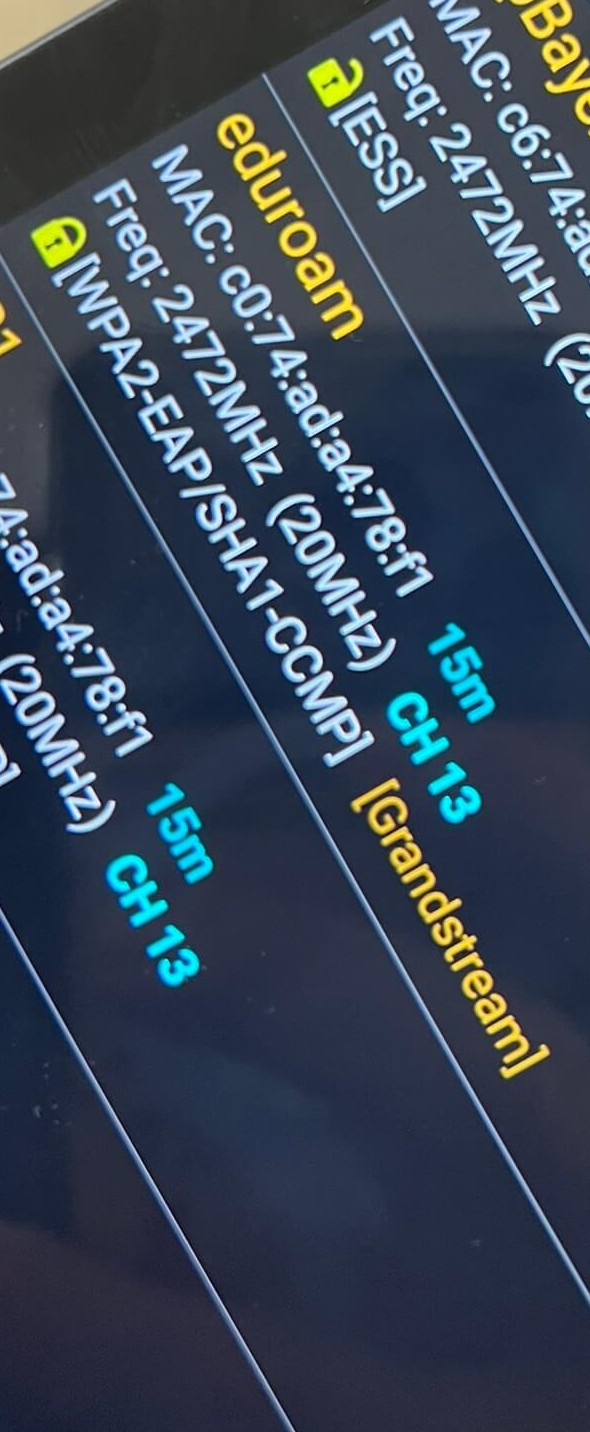
\includegraphics[width=0.25\textwidth]{figures/rssi-ssid.jpg}
    \caption{MAC Adresse des für Aufgabe \ref{sec:rssi} verwendeten APs.}
    \label{rssi-mac}
\end{figure}

\begin{figure}[h]
    \centering
    \begin{minipage}{.6\textwidth}
        \centering
        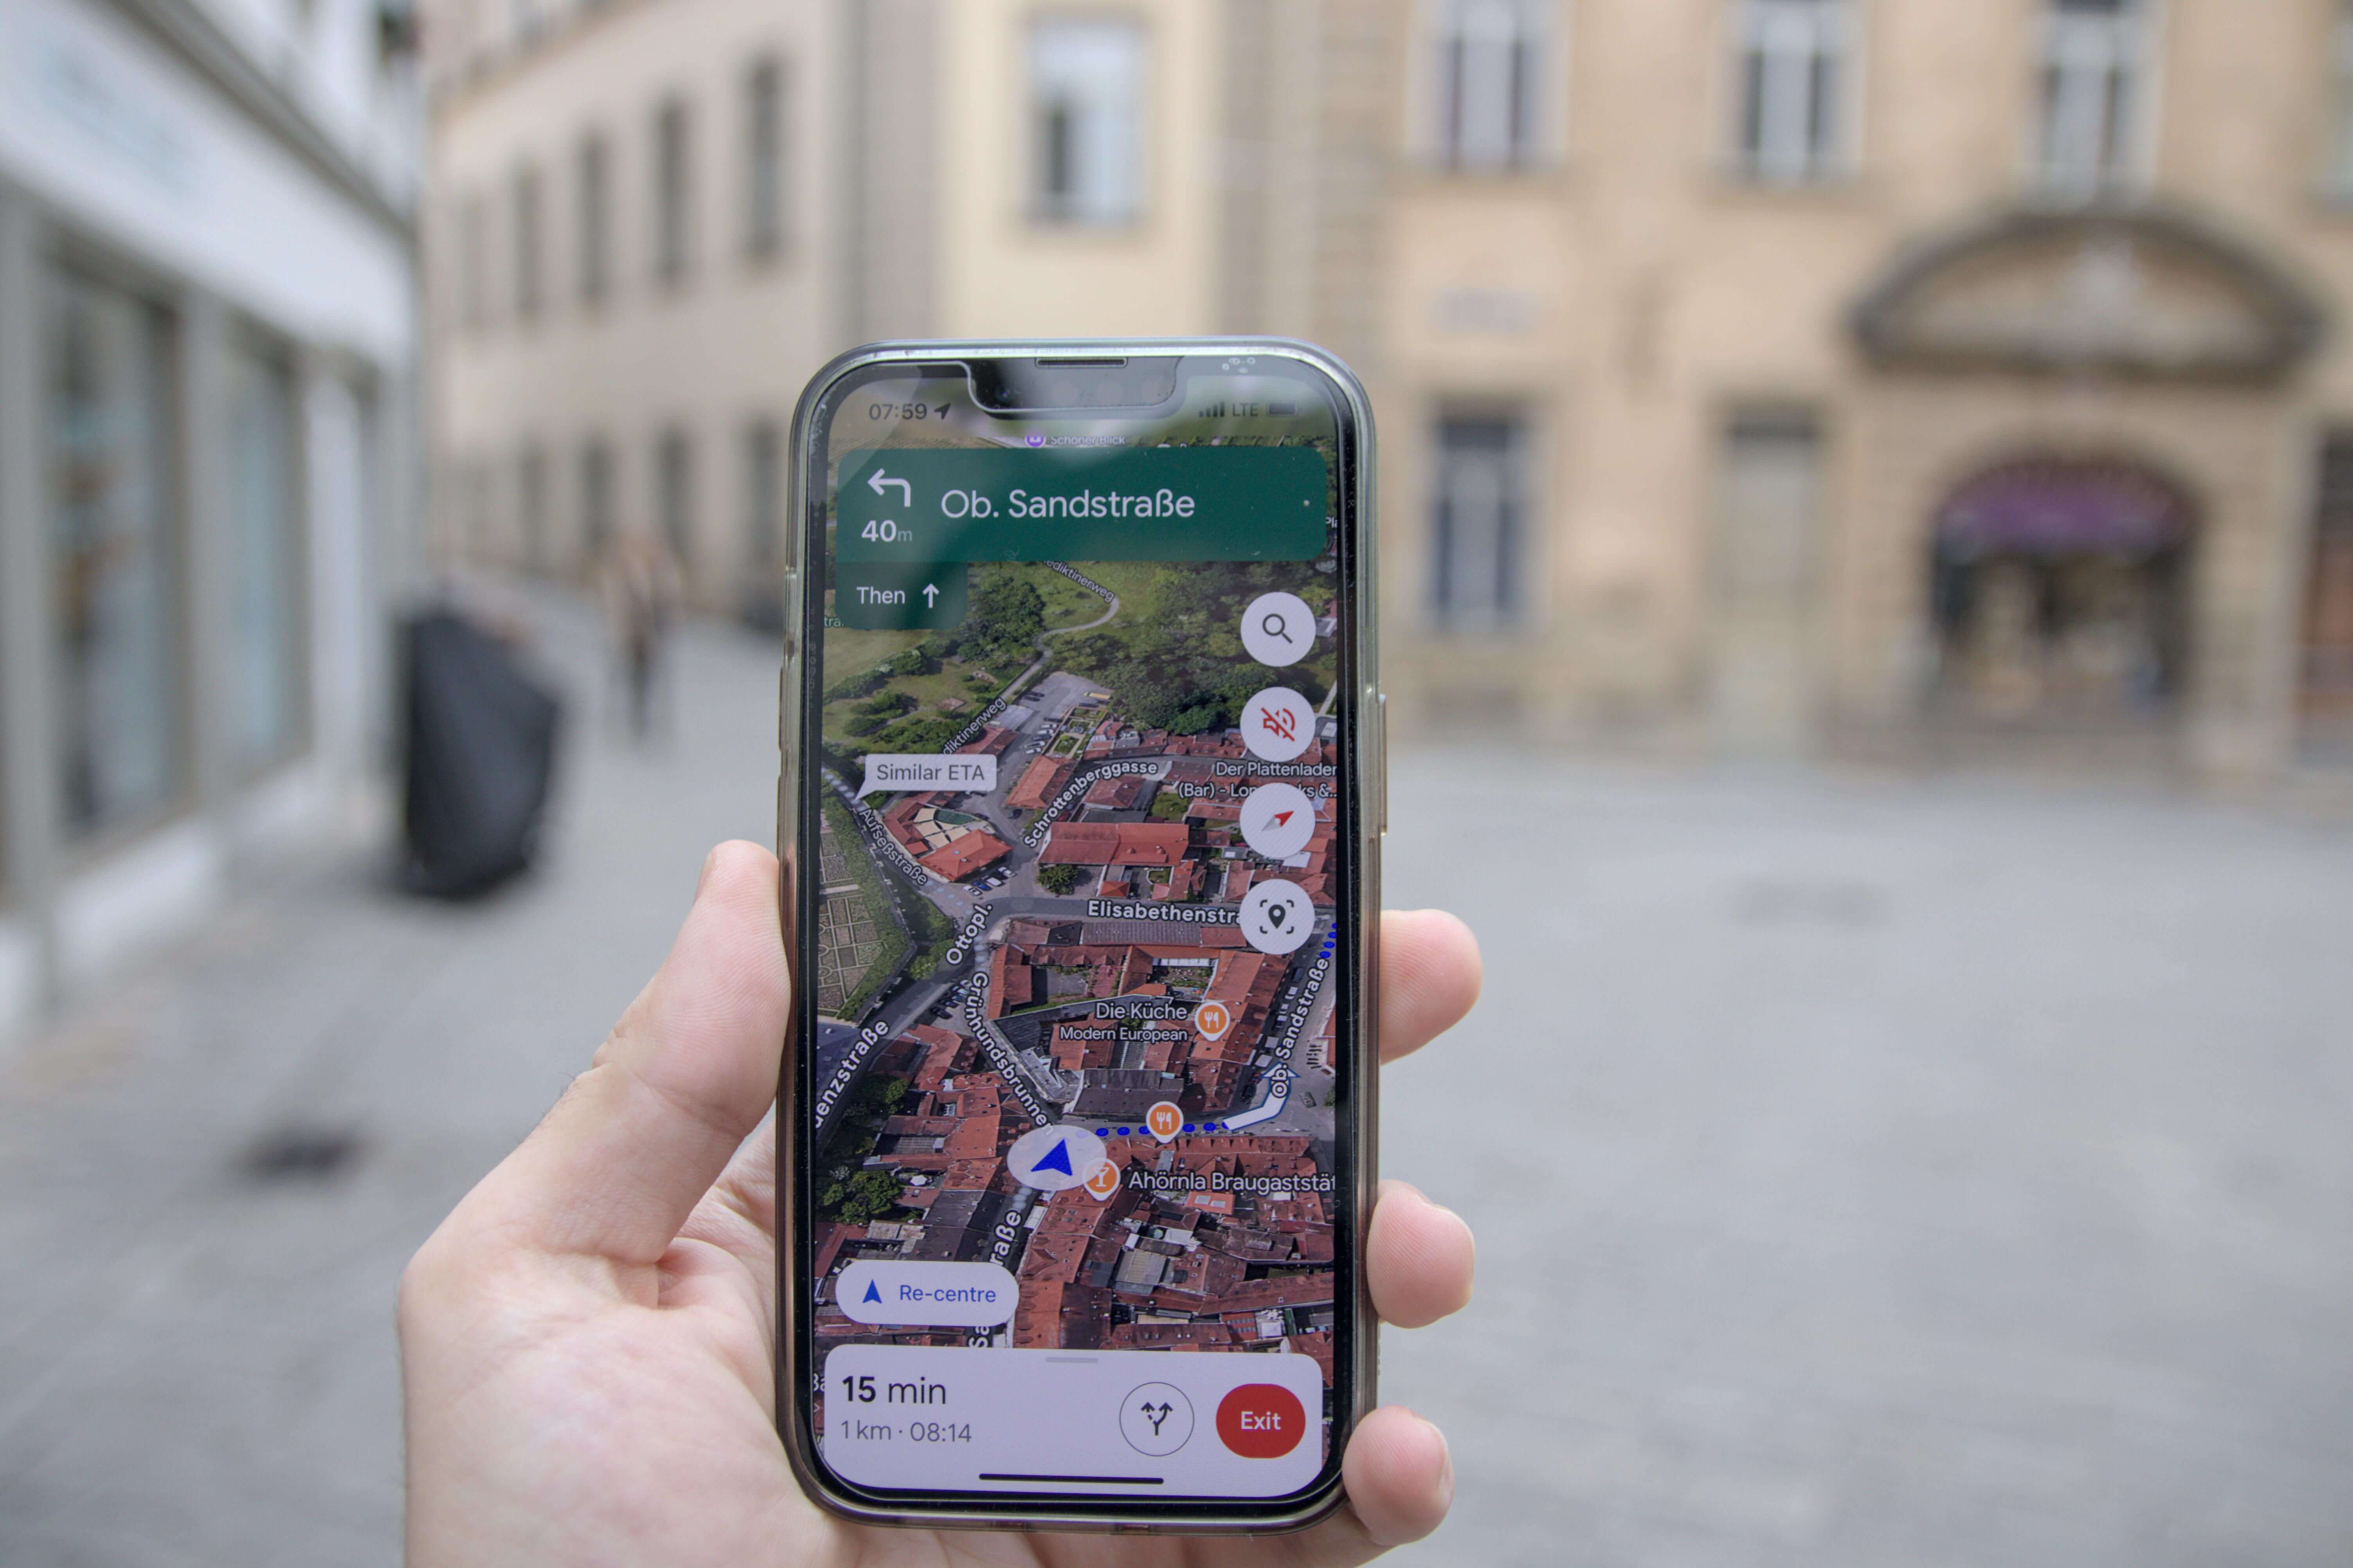
\includegraphics[width=\linewidth]{figures/geocaching/first/IMG_3087.jpg}
    \end{minipage}%
    \begin{minipage}{.4\textwidth}
        \centering
        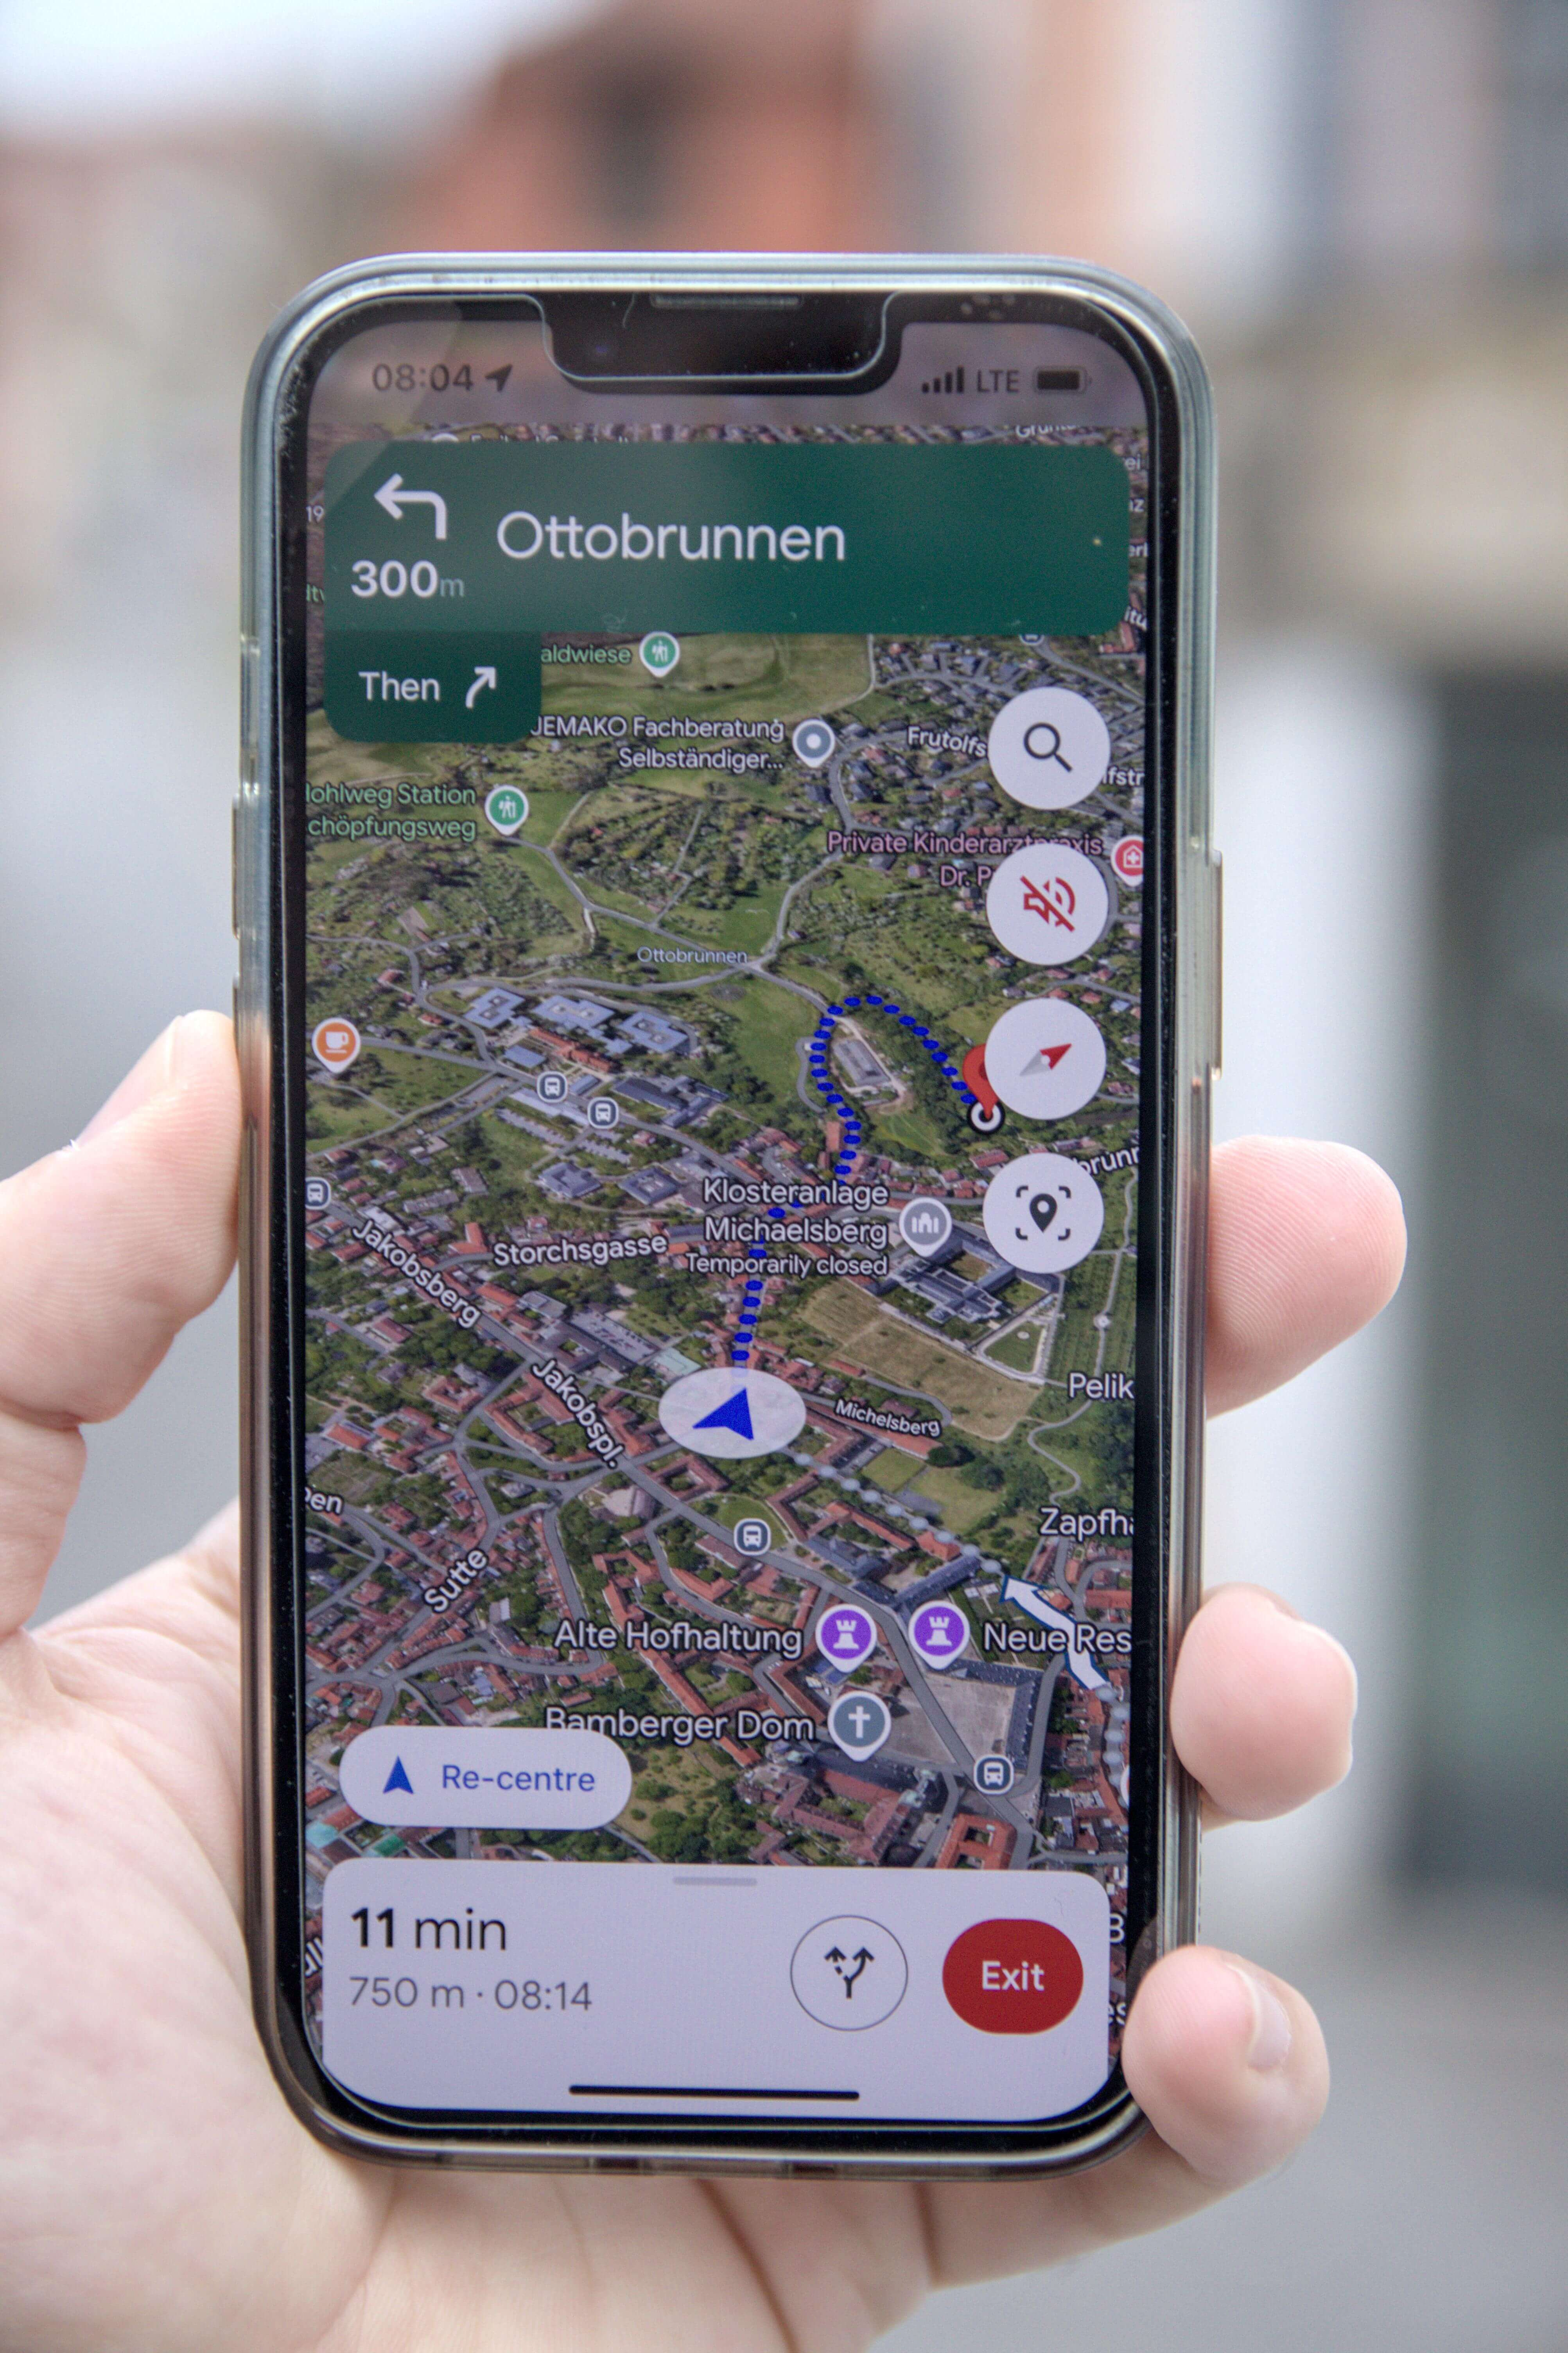
\includegraphics[width=.7\linewidth]{figures/geocaching/first/IMG_3092.jpg}
    \end{minipage}
    \caption{Auf dem Weg zum ersten Cache. In der Sandstraße entscheide ich mich für eine Alternativroute (links). Rechts: Kontrollblick auf die Navigation}
    \label{first-cache-way}
\end{figure}

\begin{figure}[h]
    \centering
    \begin{minipage}{.5\textwidth}
        \centering
        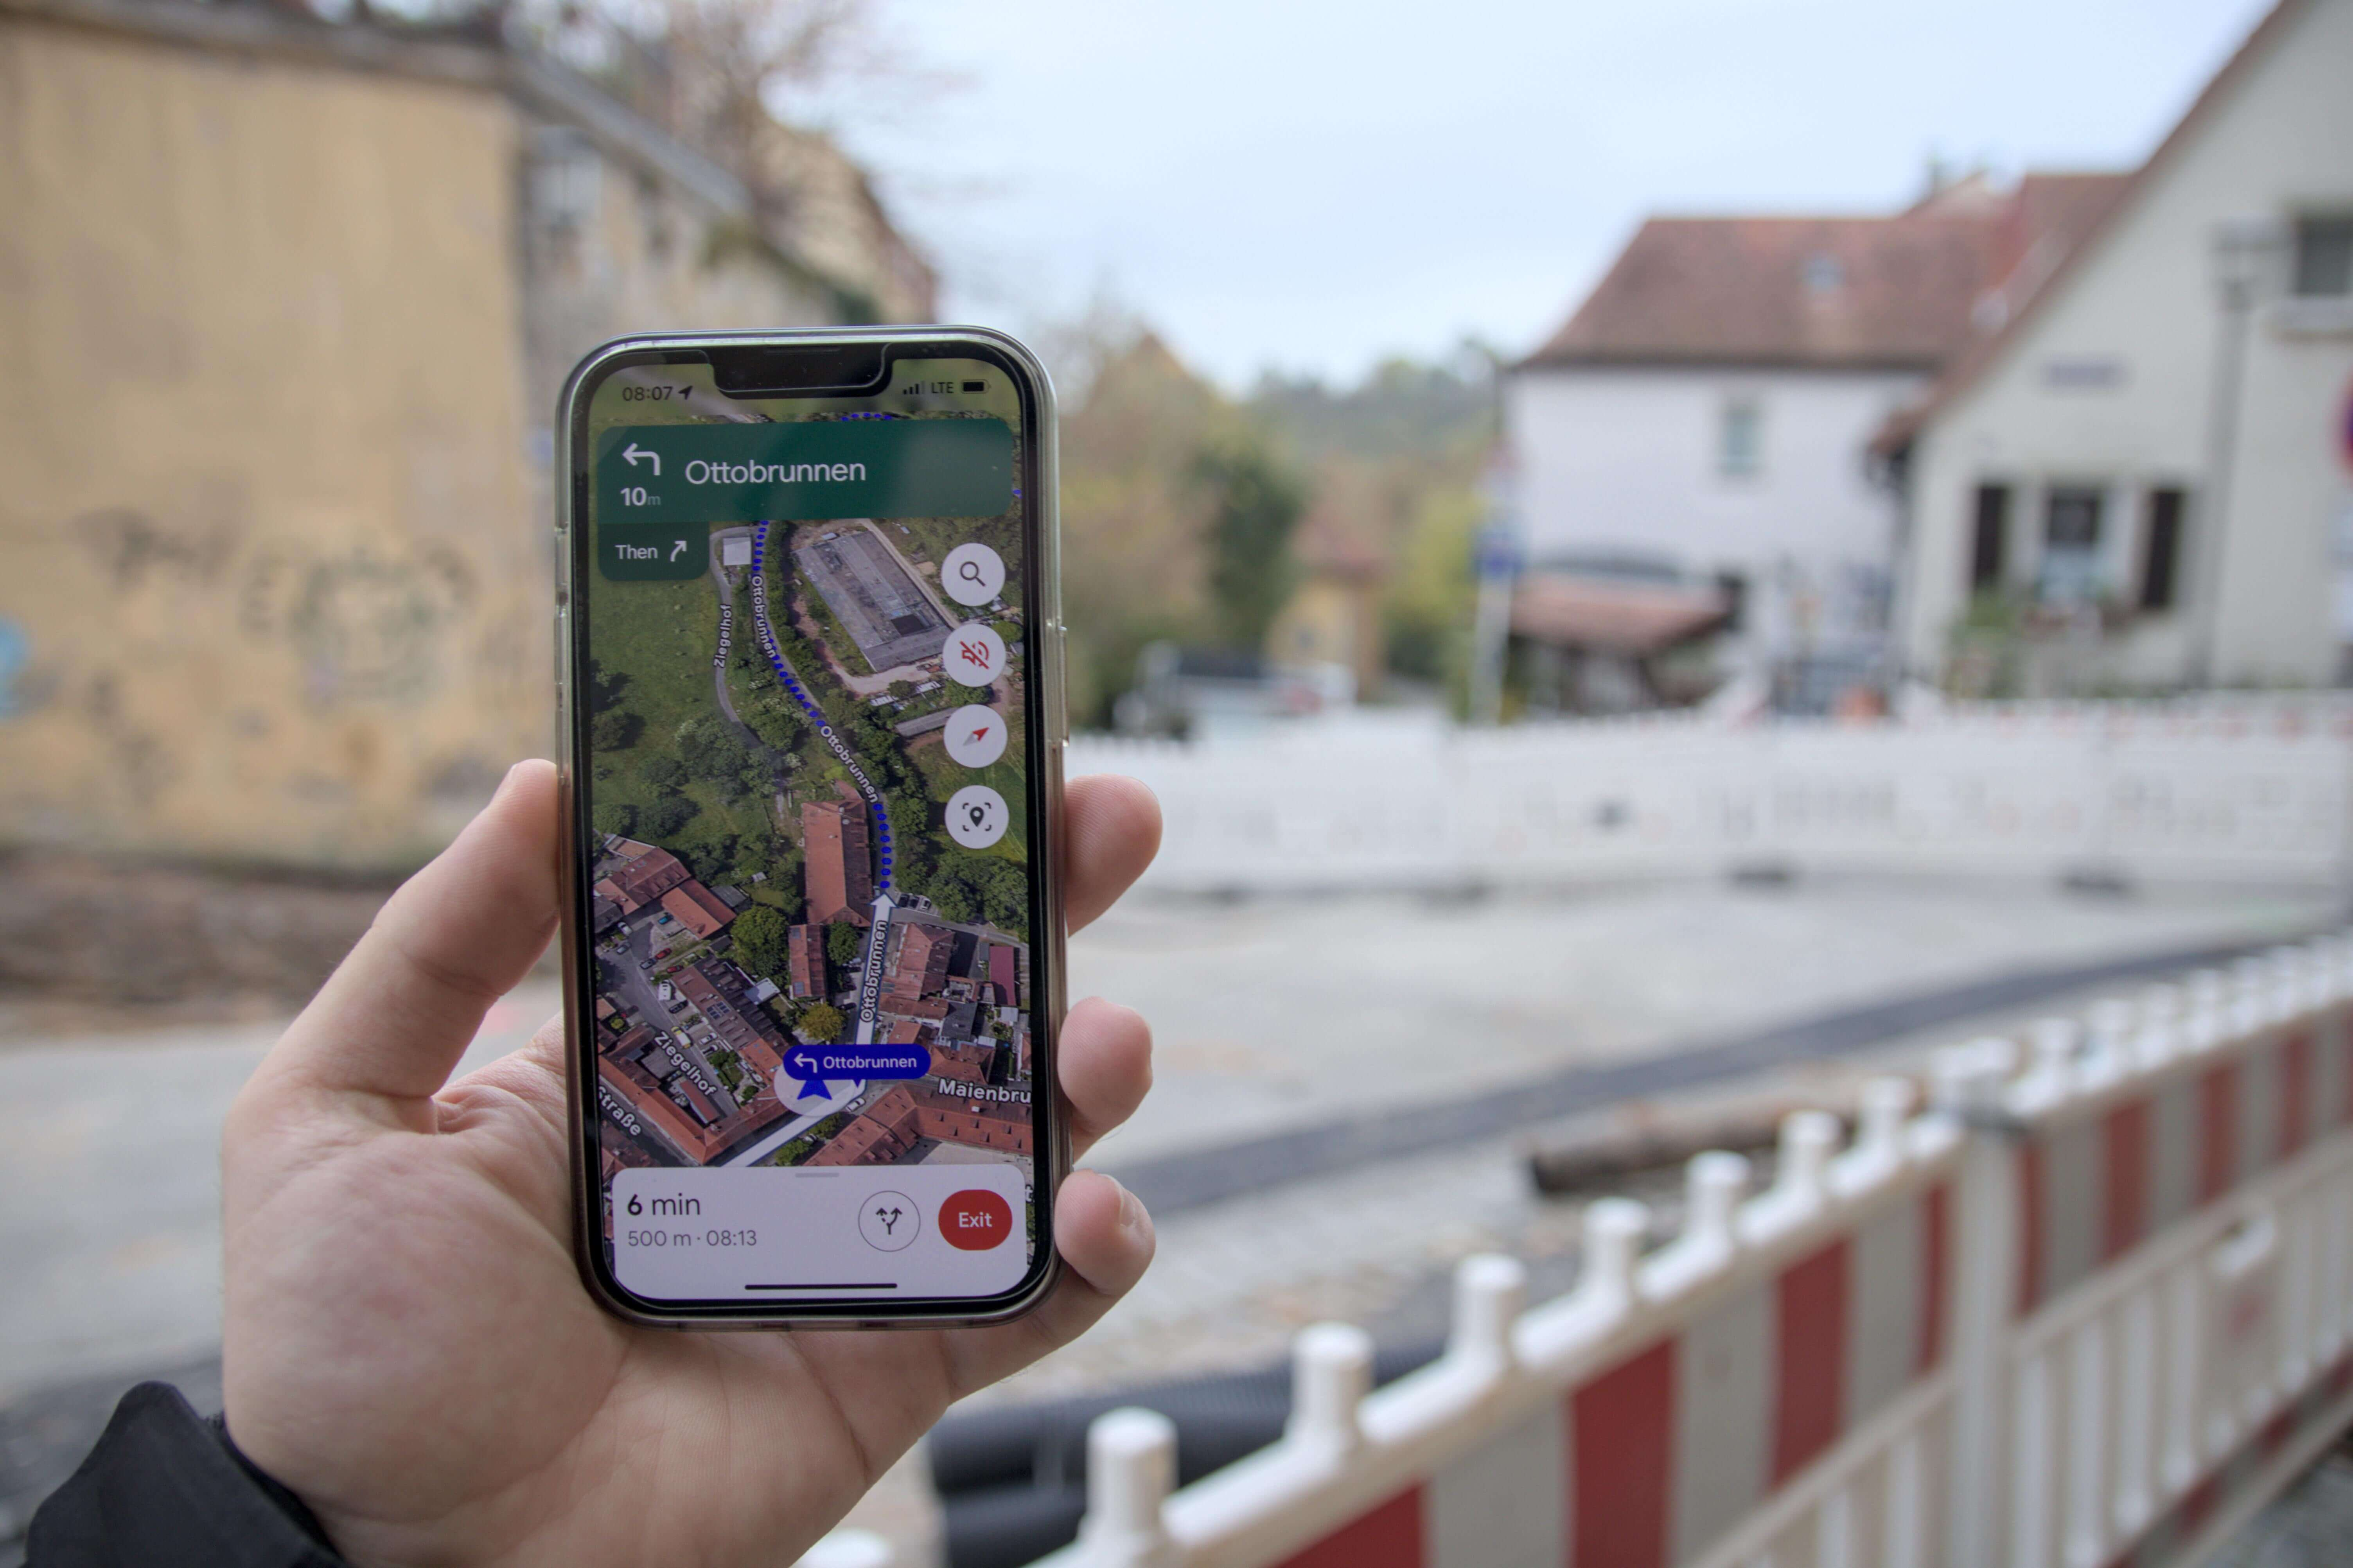
\includegraphics[width=.95\linewidth]{figures/geocaching/first/IMG_3093.jpg}
    \end{minipage}%
    \begin{minipage}{.5\textwidth}
        \centering
        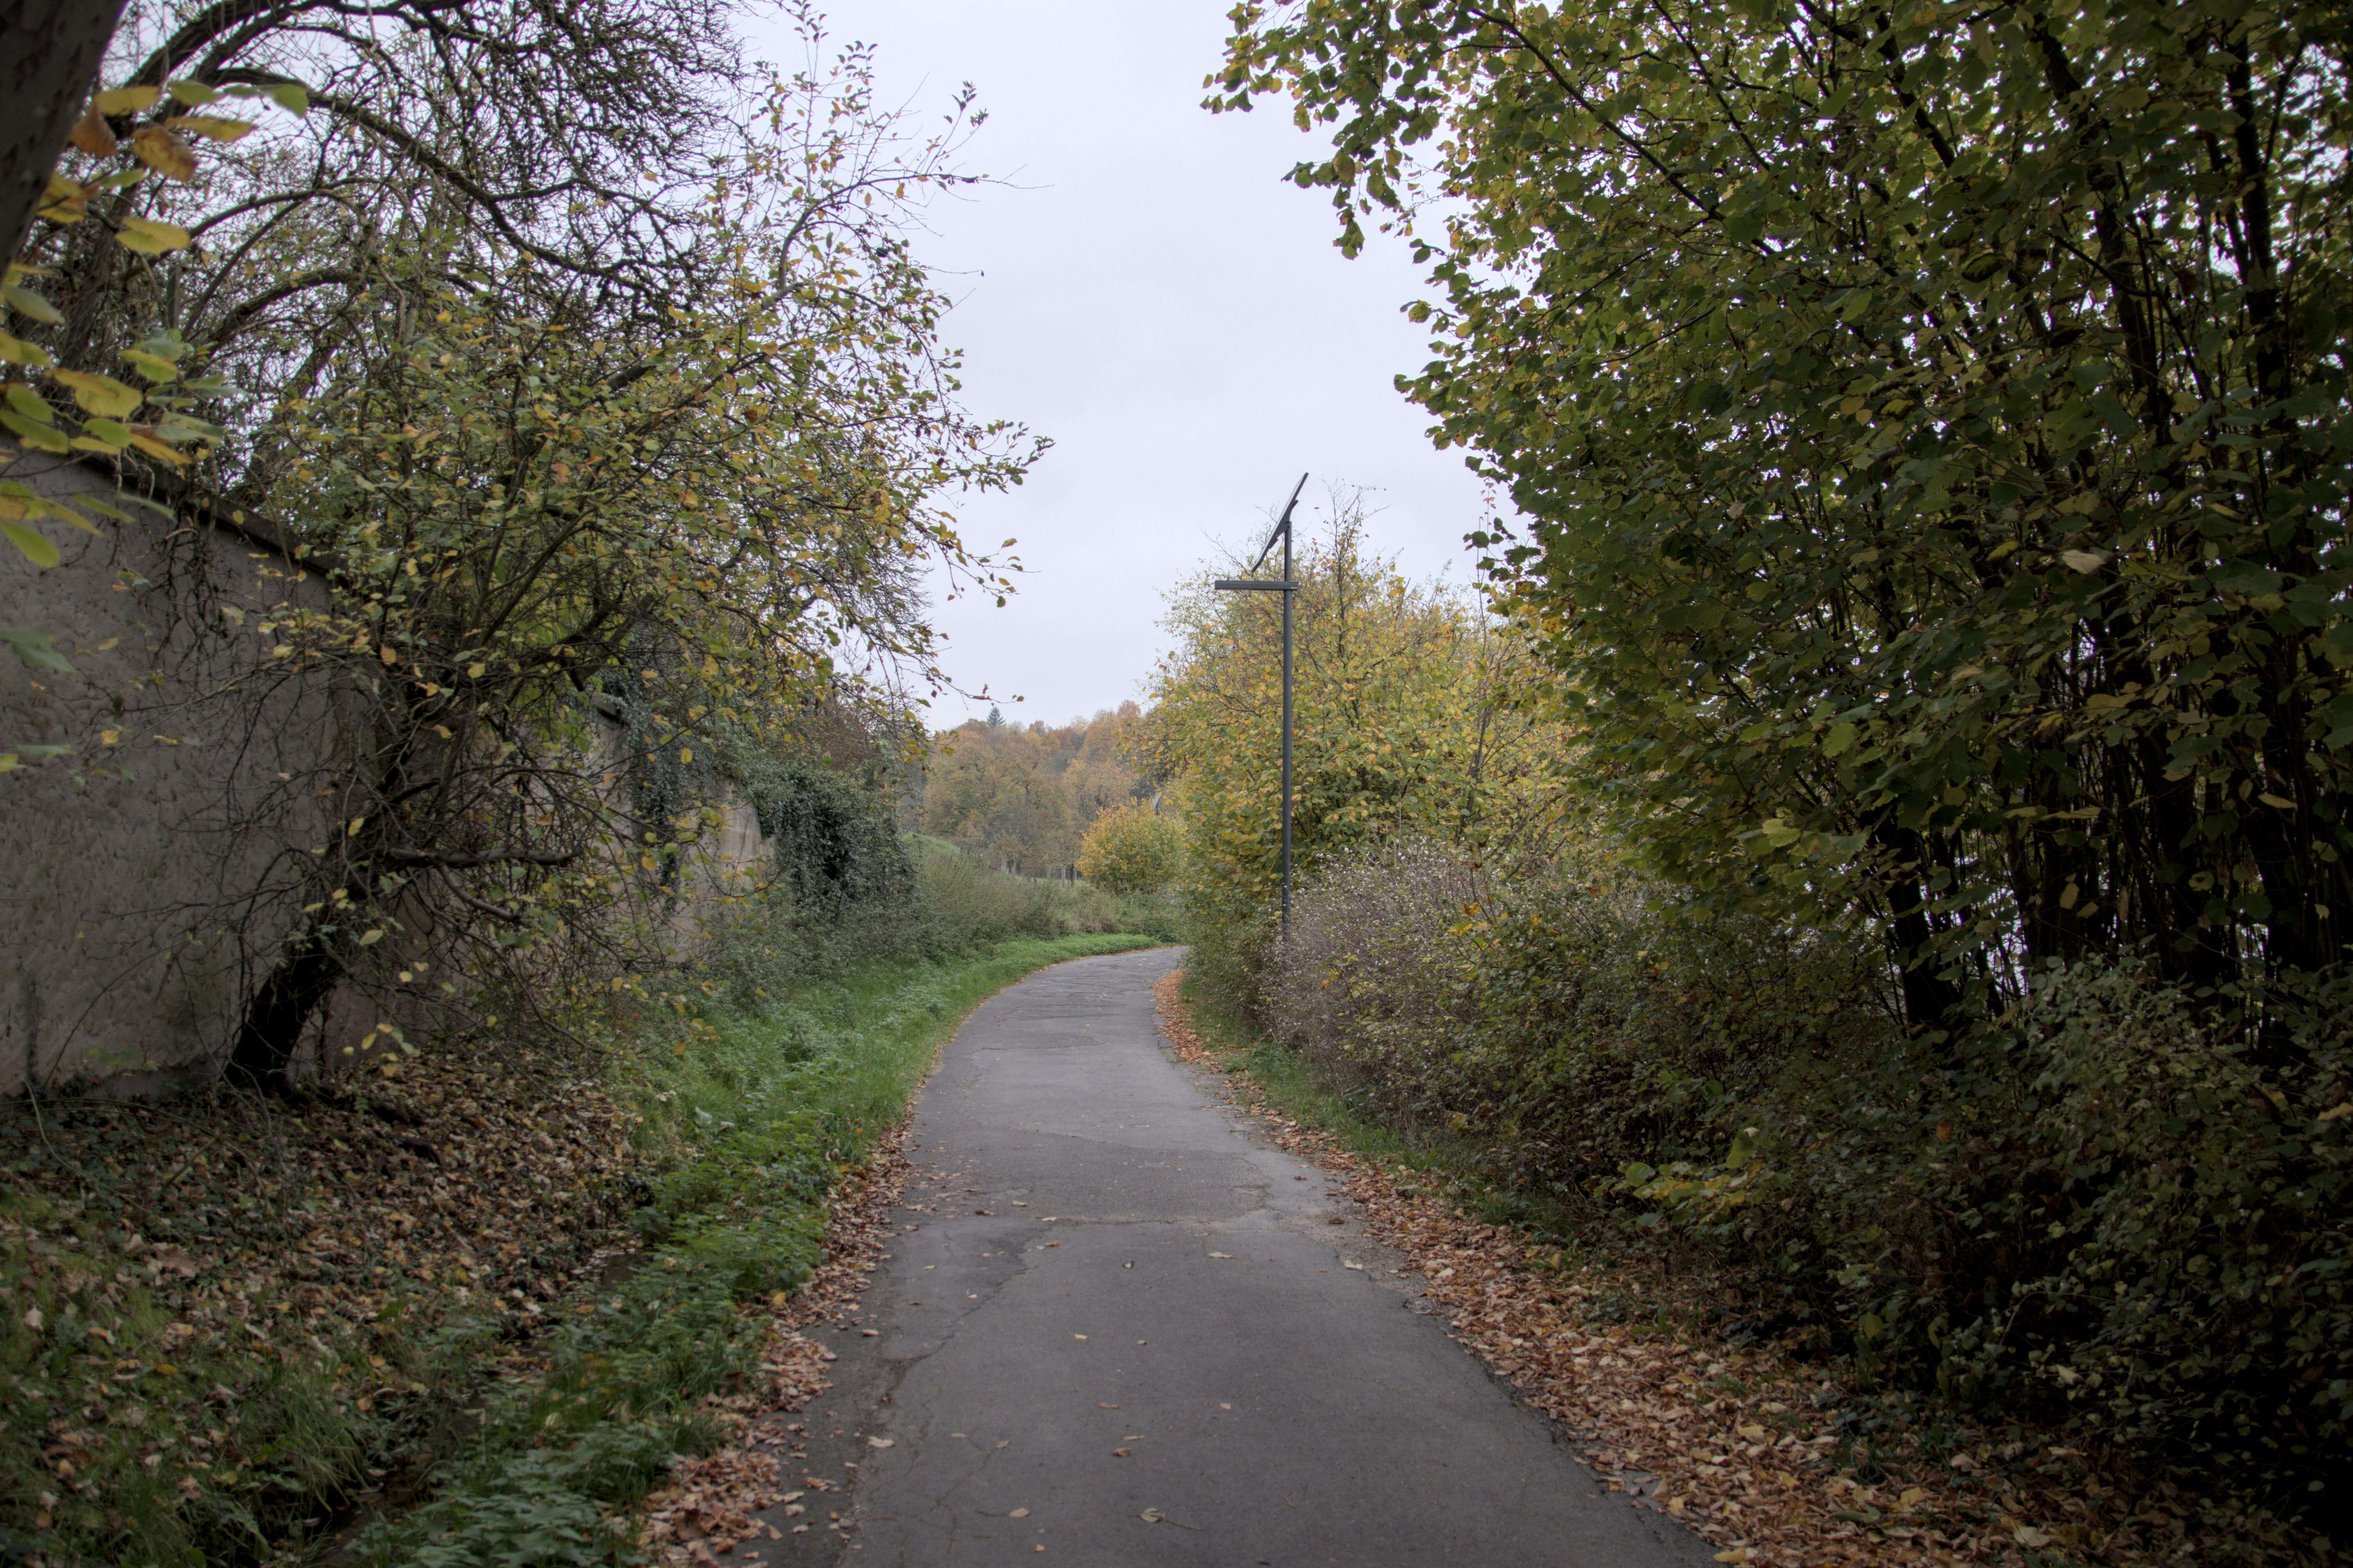
\includegraphics[width=.95\linewidth]{figures/geocaching/first/IMG_3095.jpg}
    \end{minipage}
    \caption{Kaum ist die Baustelle überwunden, bin ich praktisch raus aus der Stadt.}
    \label{first-cache-baustelle}
\end{figure}

\begin{figure}[h]
    \centering
    \begin{minipage}{.4\textwidth}
        \centering
        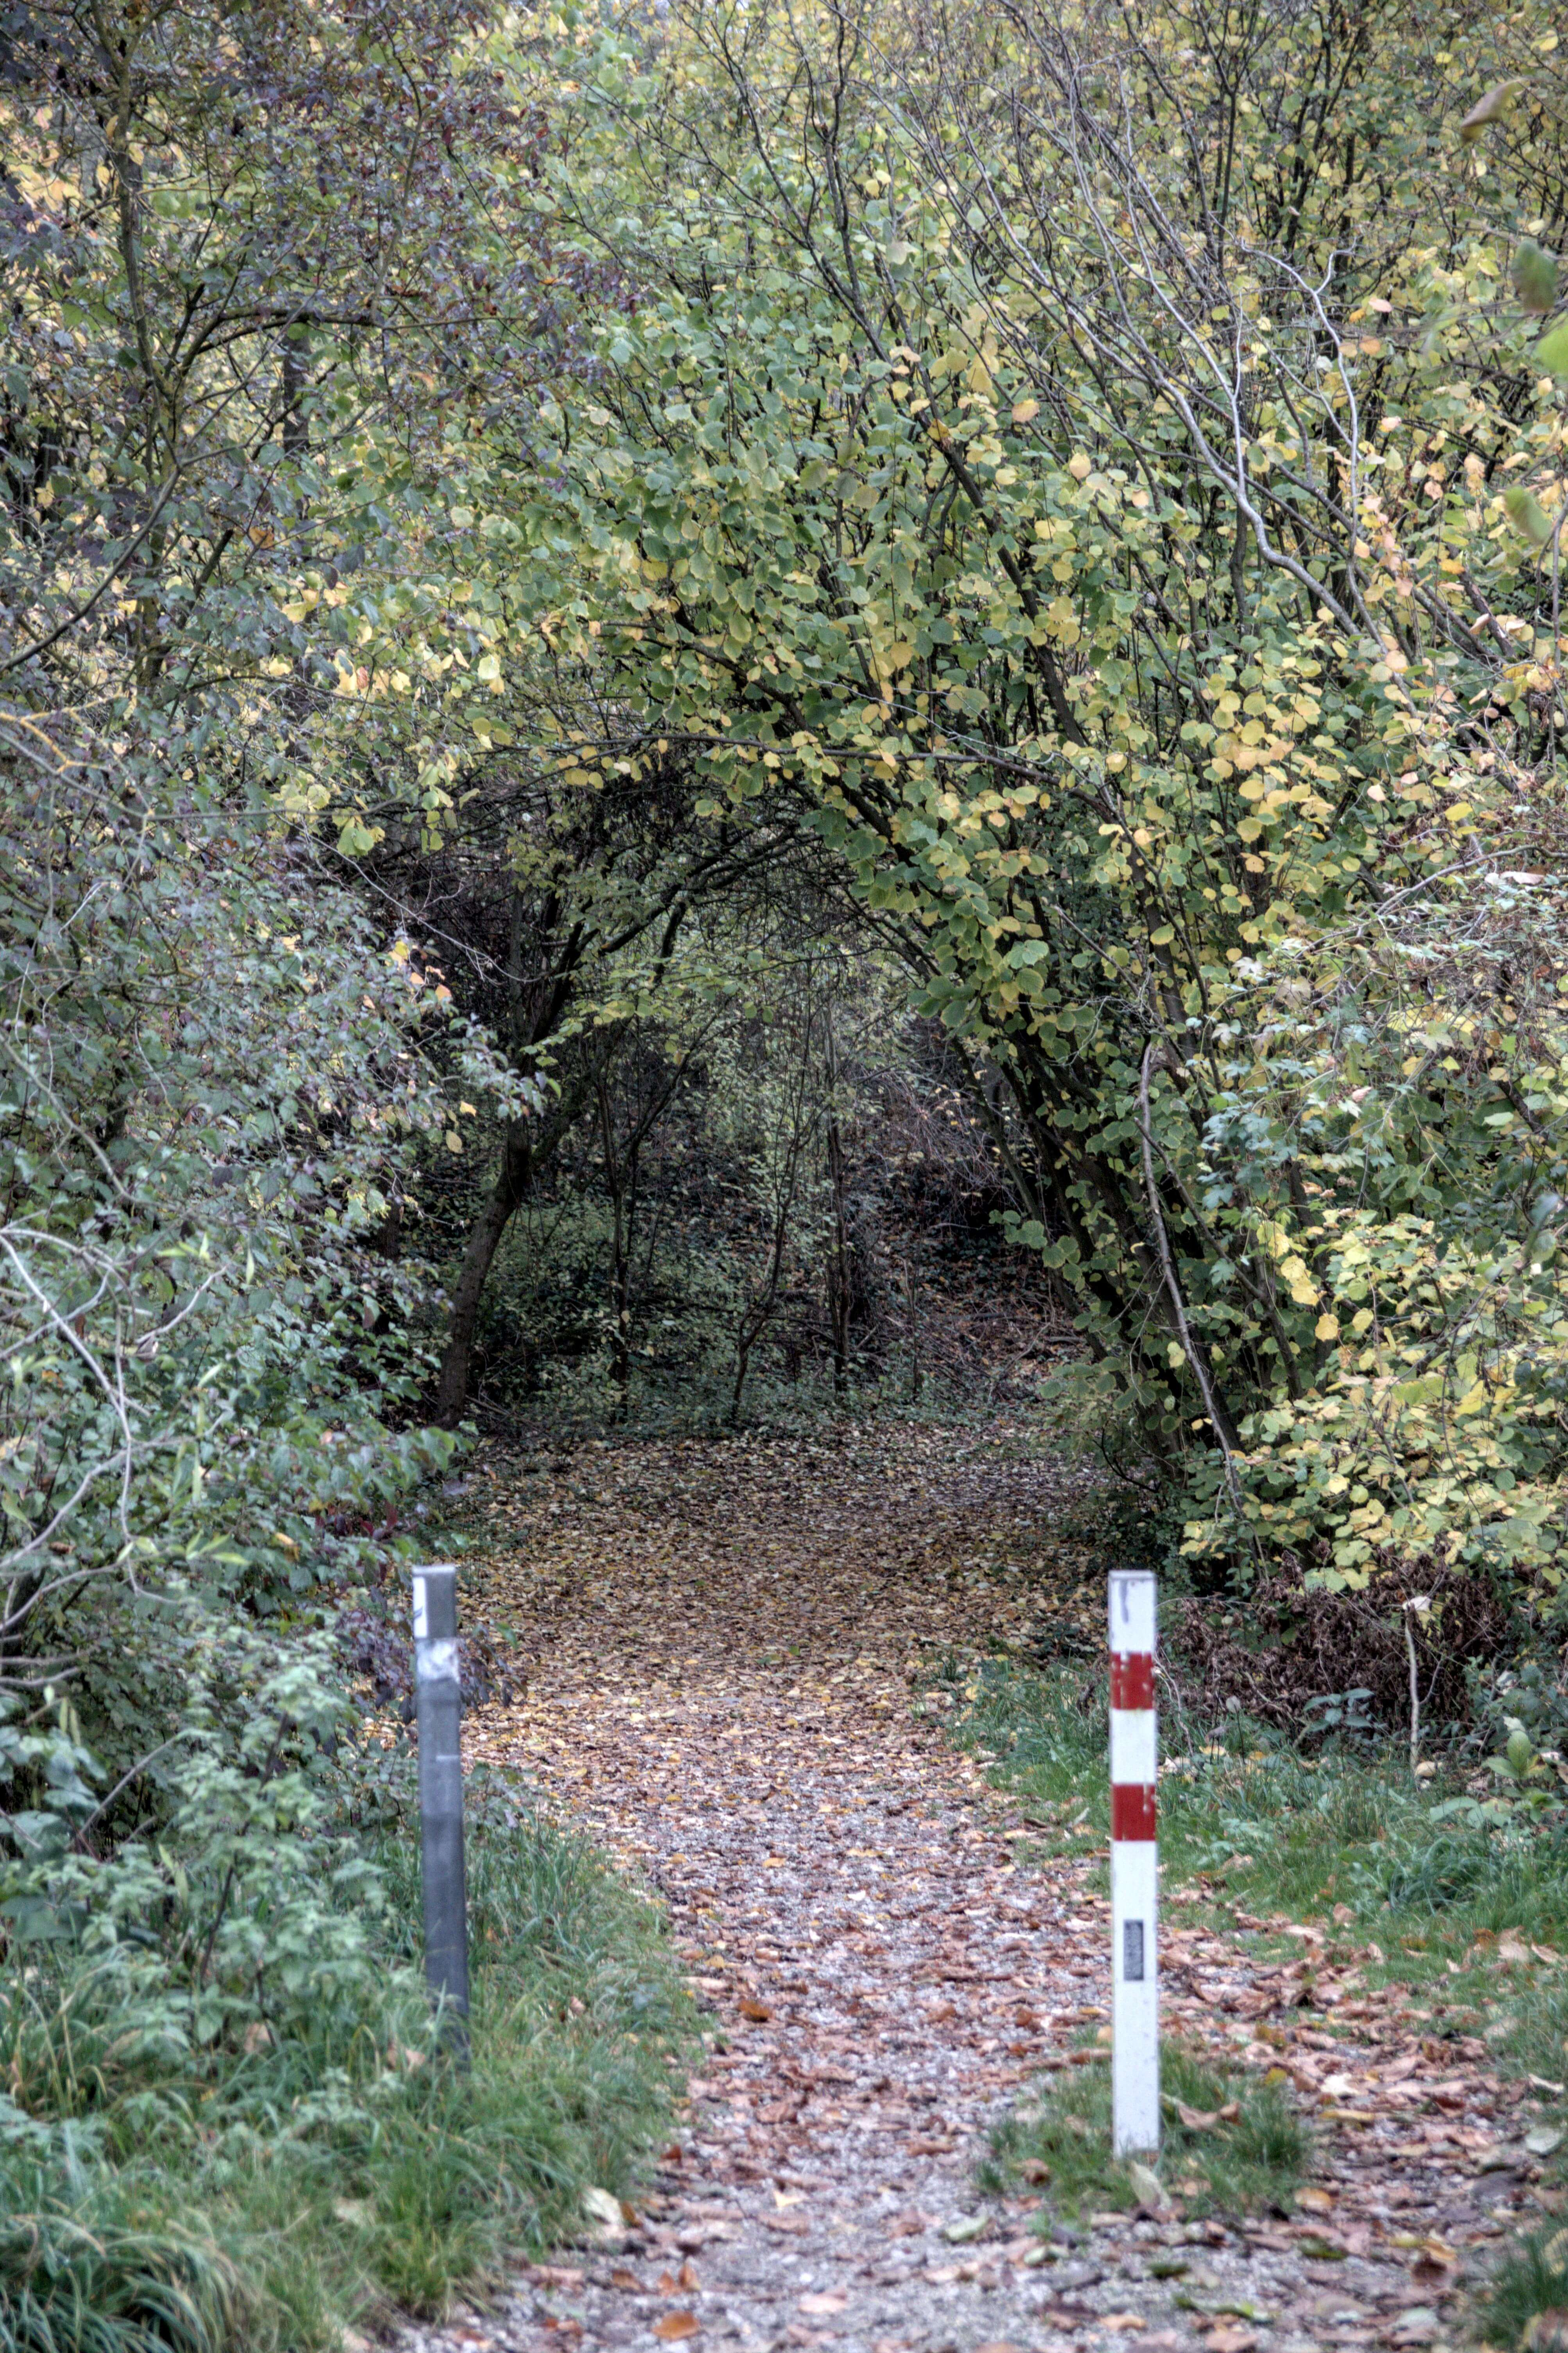
\includegraphics[width=.7\linewidth]{figures/geocaching/first/IMG_3096.jpg}
    \end{minipage}%
    \begin{minipage}{.6\textwidth}
        \centering
        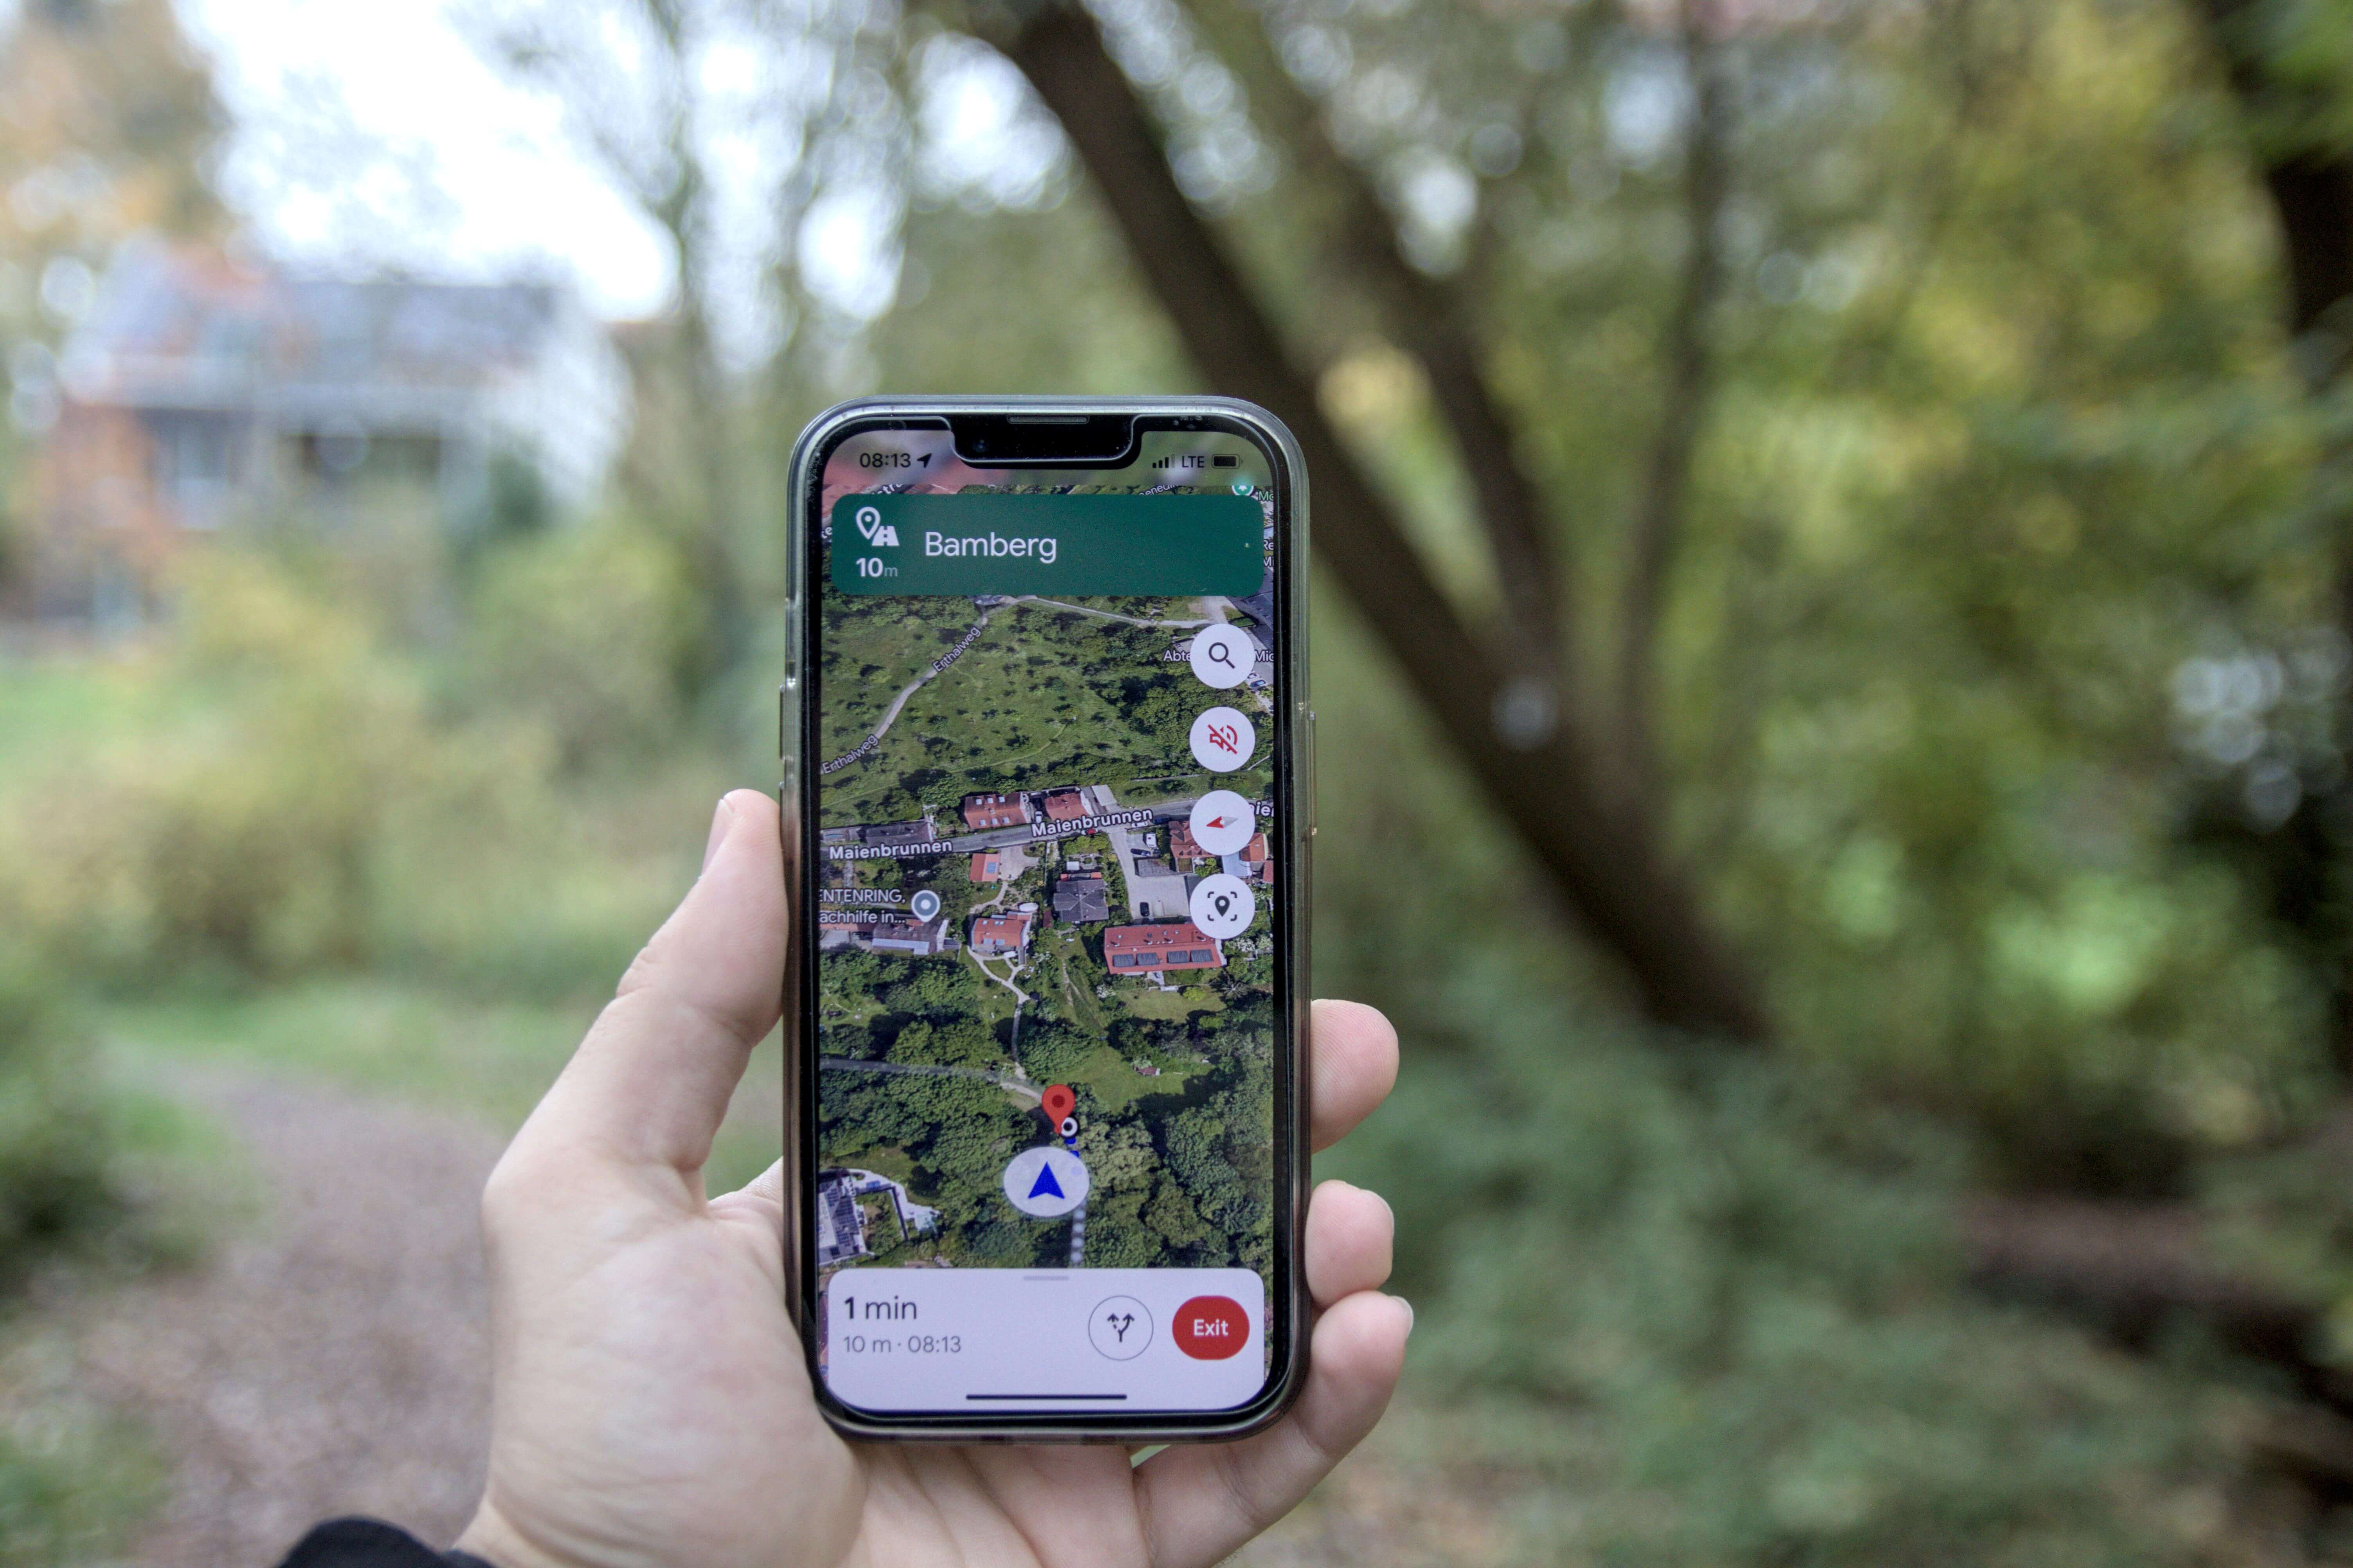
\includegraphics[width=\linewidth]{figures/geocaching/first/IMG_3098.jpg}
    \end{minipage}
    \caption{Ich folge einem unscheinbaren Weg hinab in den Jungle. Einige hundert Meter später bin ich am Ziel.}
    \label{first-cache-ziel}
\end{figure}

\begin{figure}[h]
    \centering
    \begin{minipage}{.5\textwidth}
        \centering
        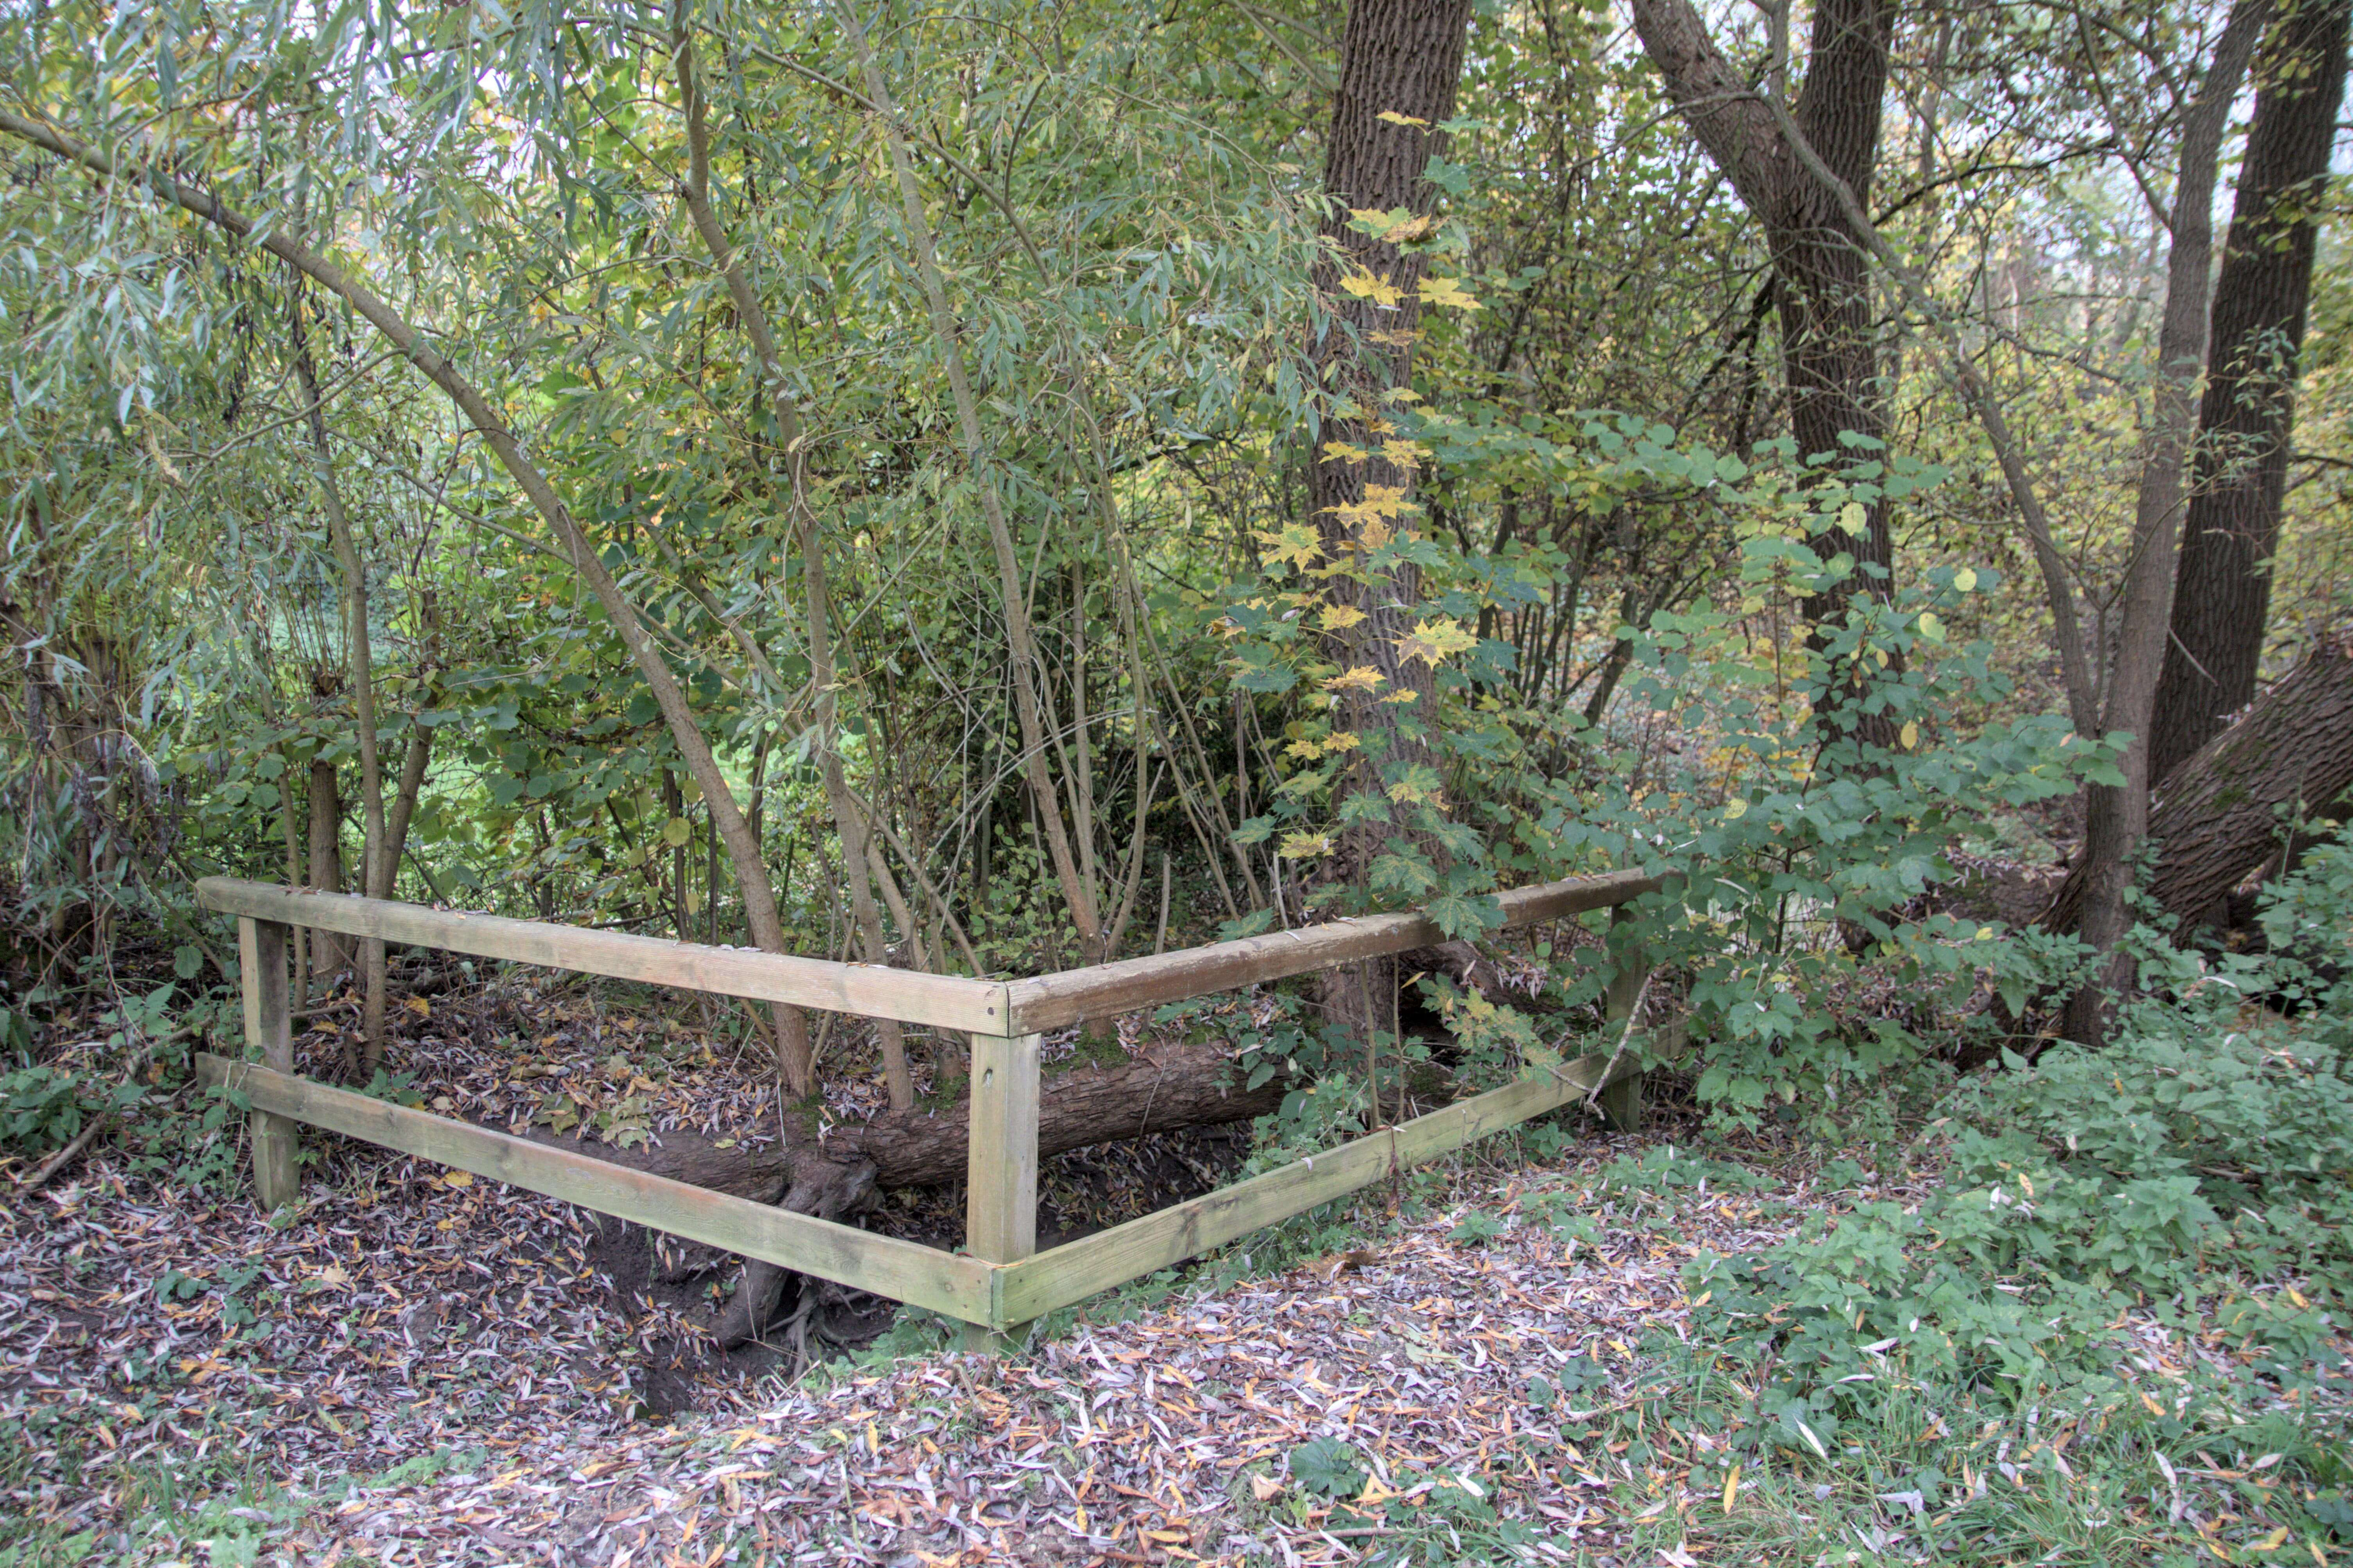
\includegraphics[width=.95\linewidth]{figures/geocaching/first/IMG_3101.jpg}
    \end{minipage}%
    \begin{minipage}{.5\textwidth}
        \centering
        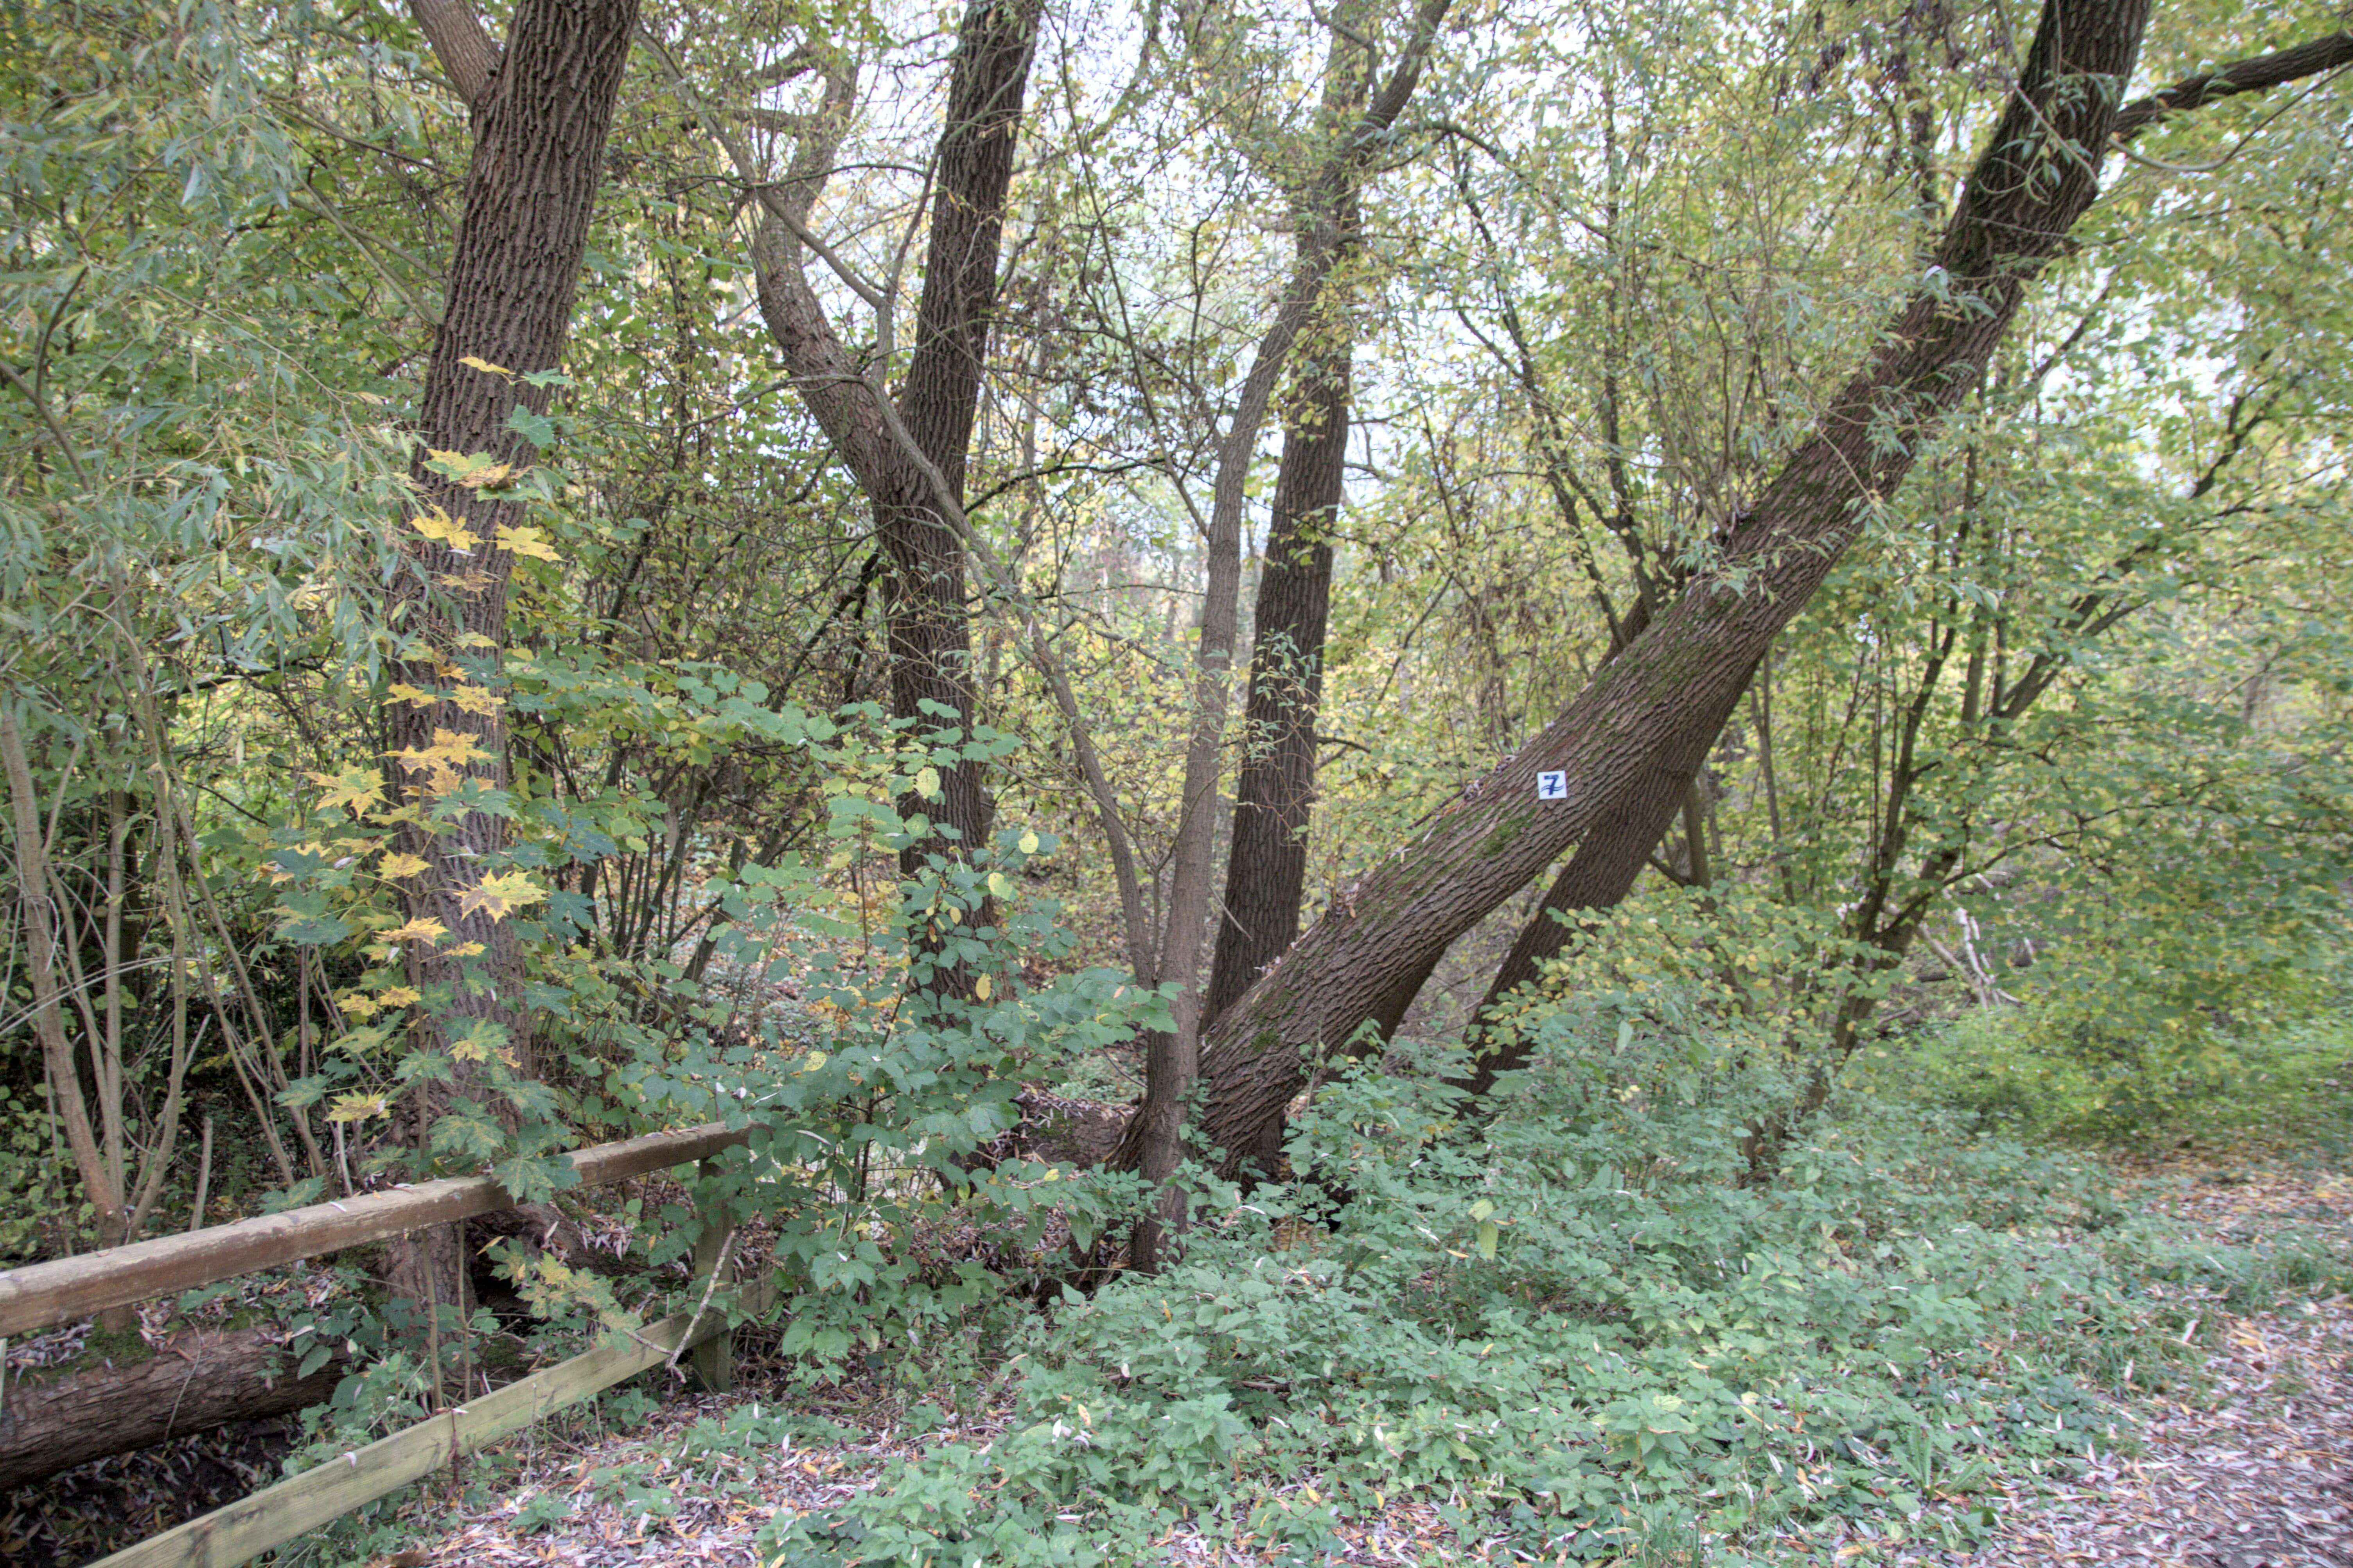
\includegraphics[width=.95\linewidth]{figures/geocaching/first/IMG_3102.jpg}
    \end{minipage}
    \caption{Links das Geländer um den Zulauf, rechts der Teich.}
    \label{first-cache-gelaende}
\end{figure}


\begin{figure}[h]
    \centering
    \begin{minipage}{.5\textwidth}
        \centering
        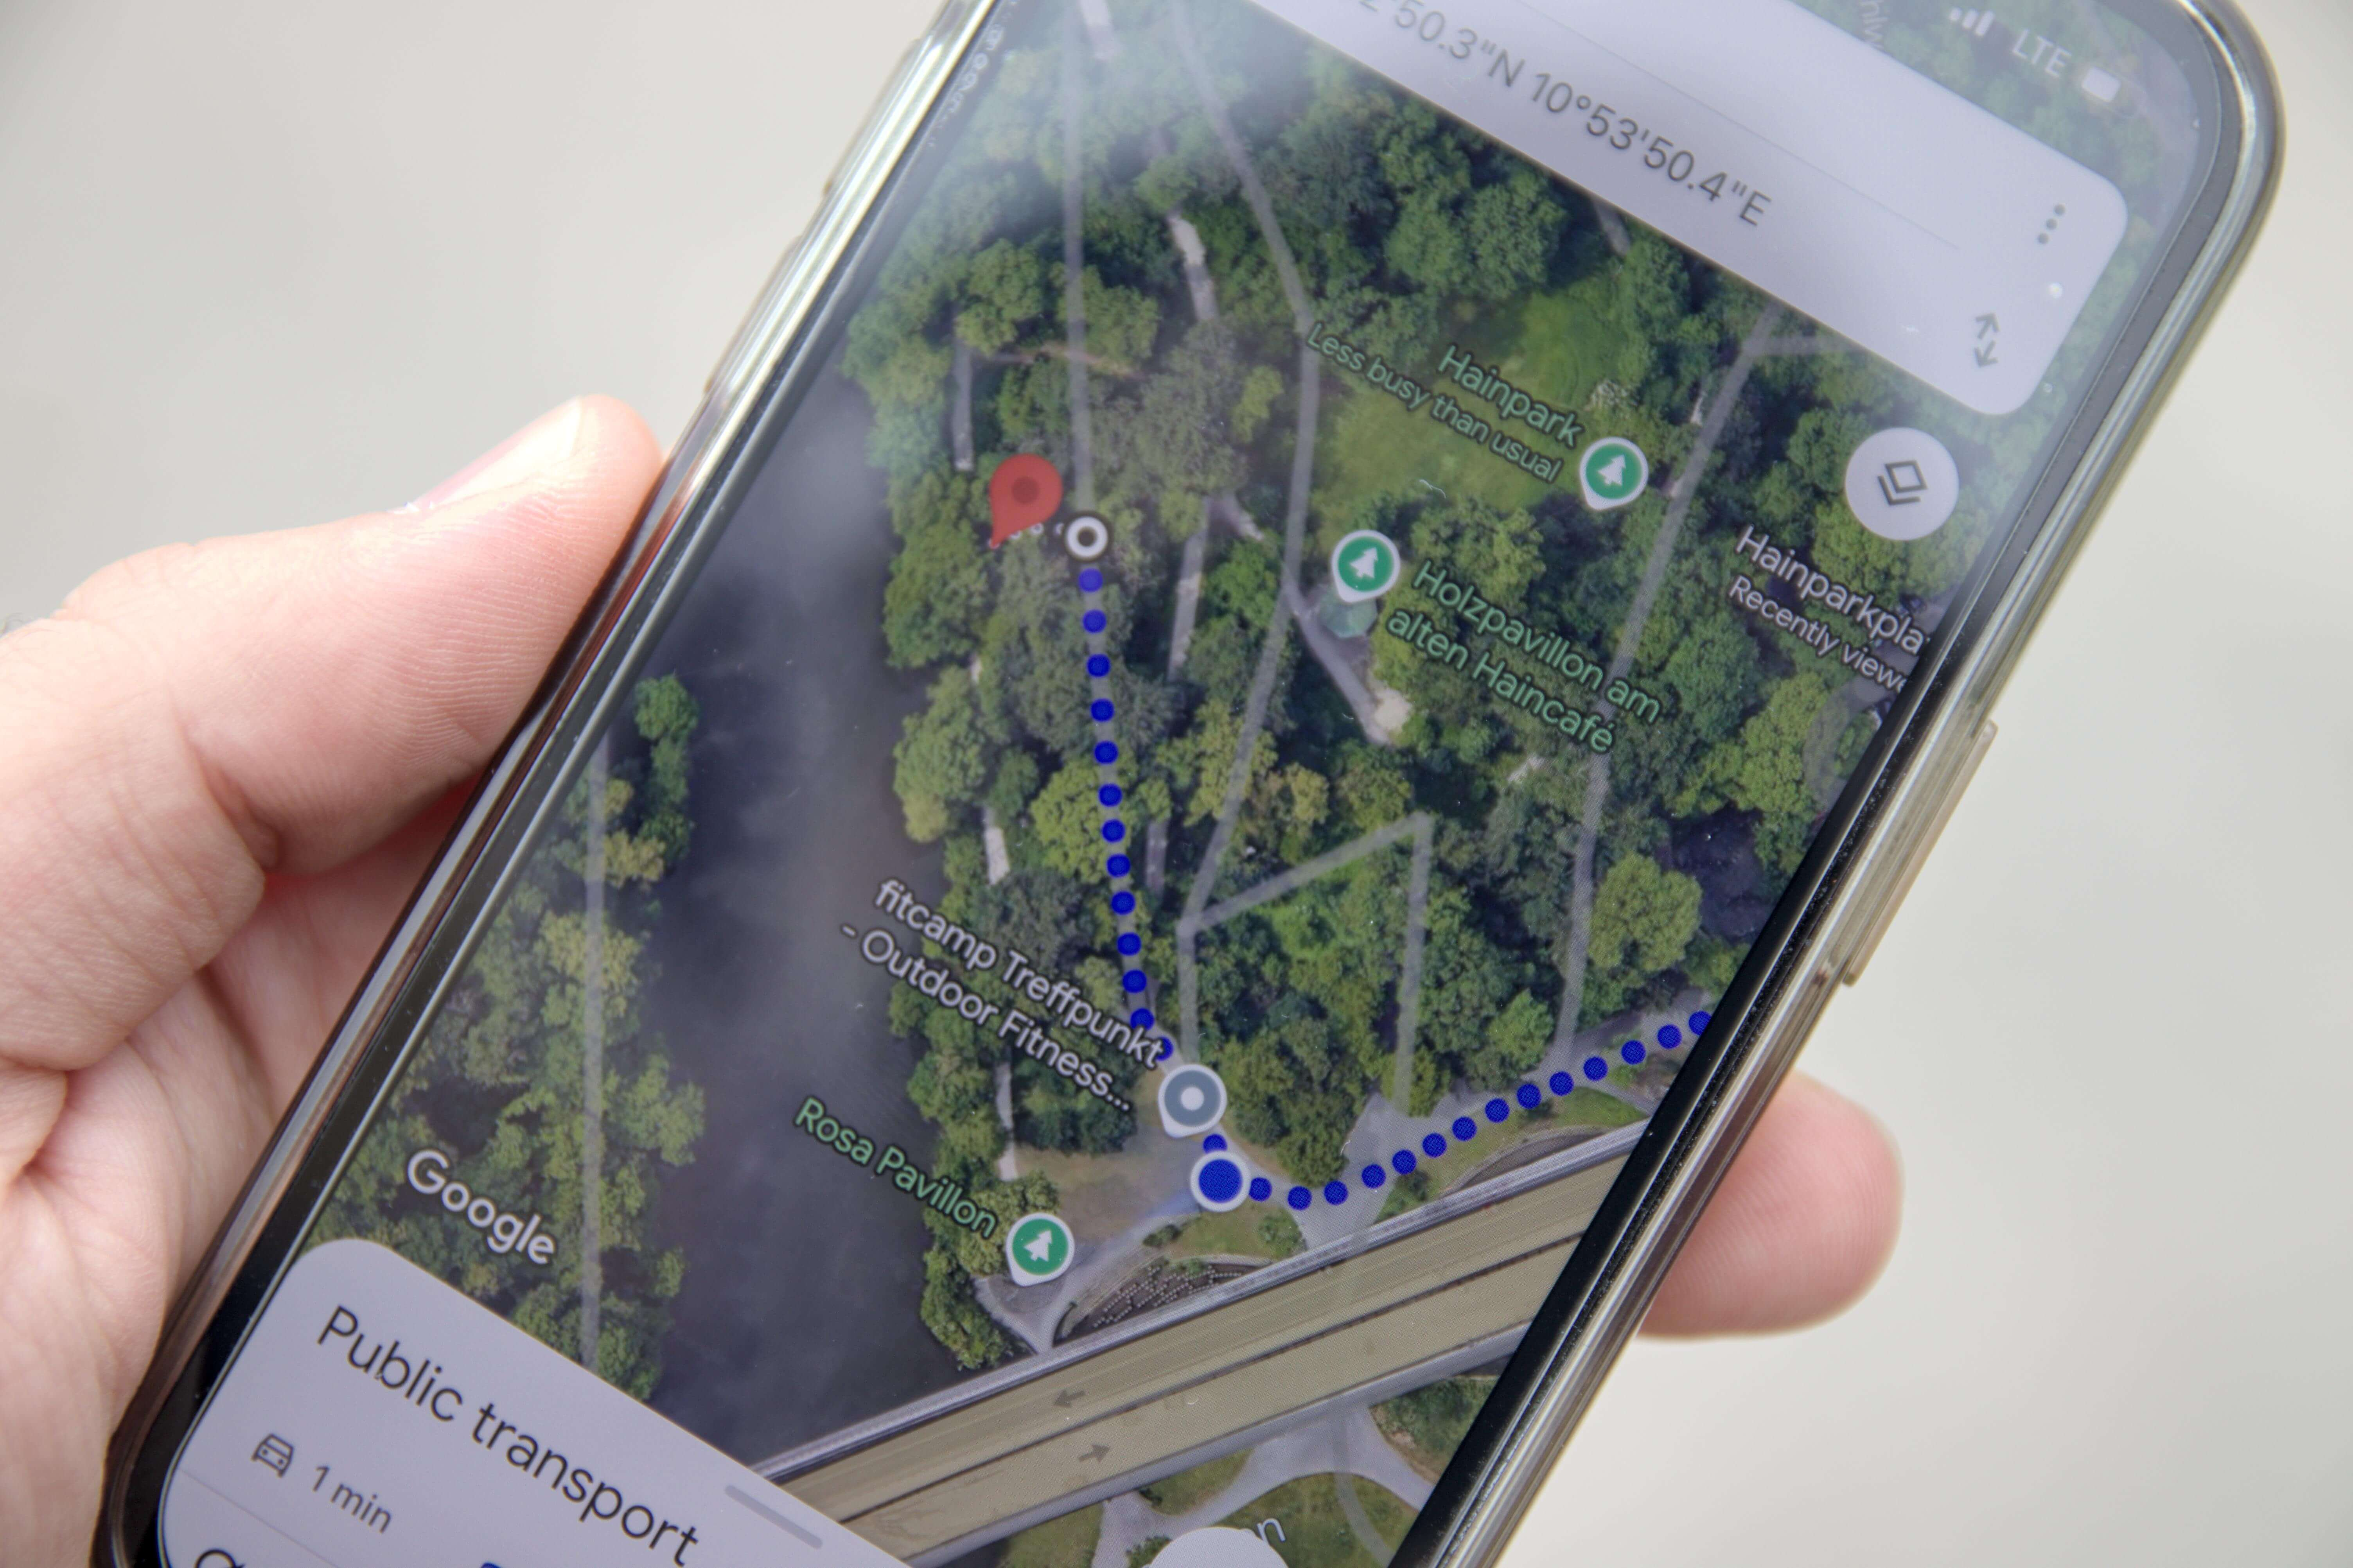
\includegraphics[width=.95\linewidth]{figures/geocaching/second/IMG_3107.jpg}
    \end{minipage}%
    \begin{minipage}{.5\textwidth}
        \centering
        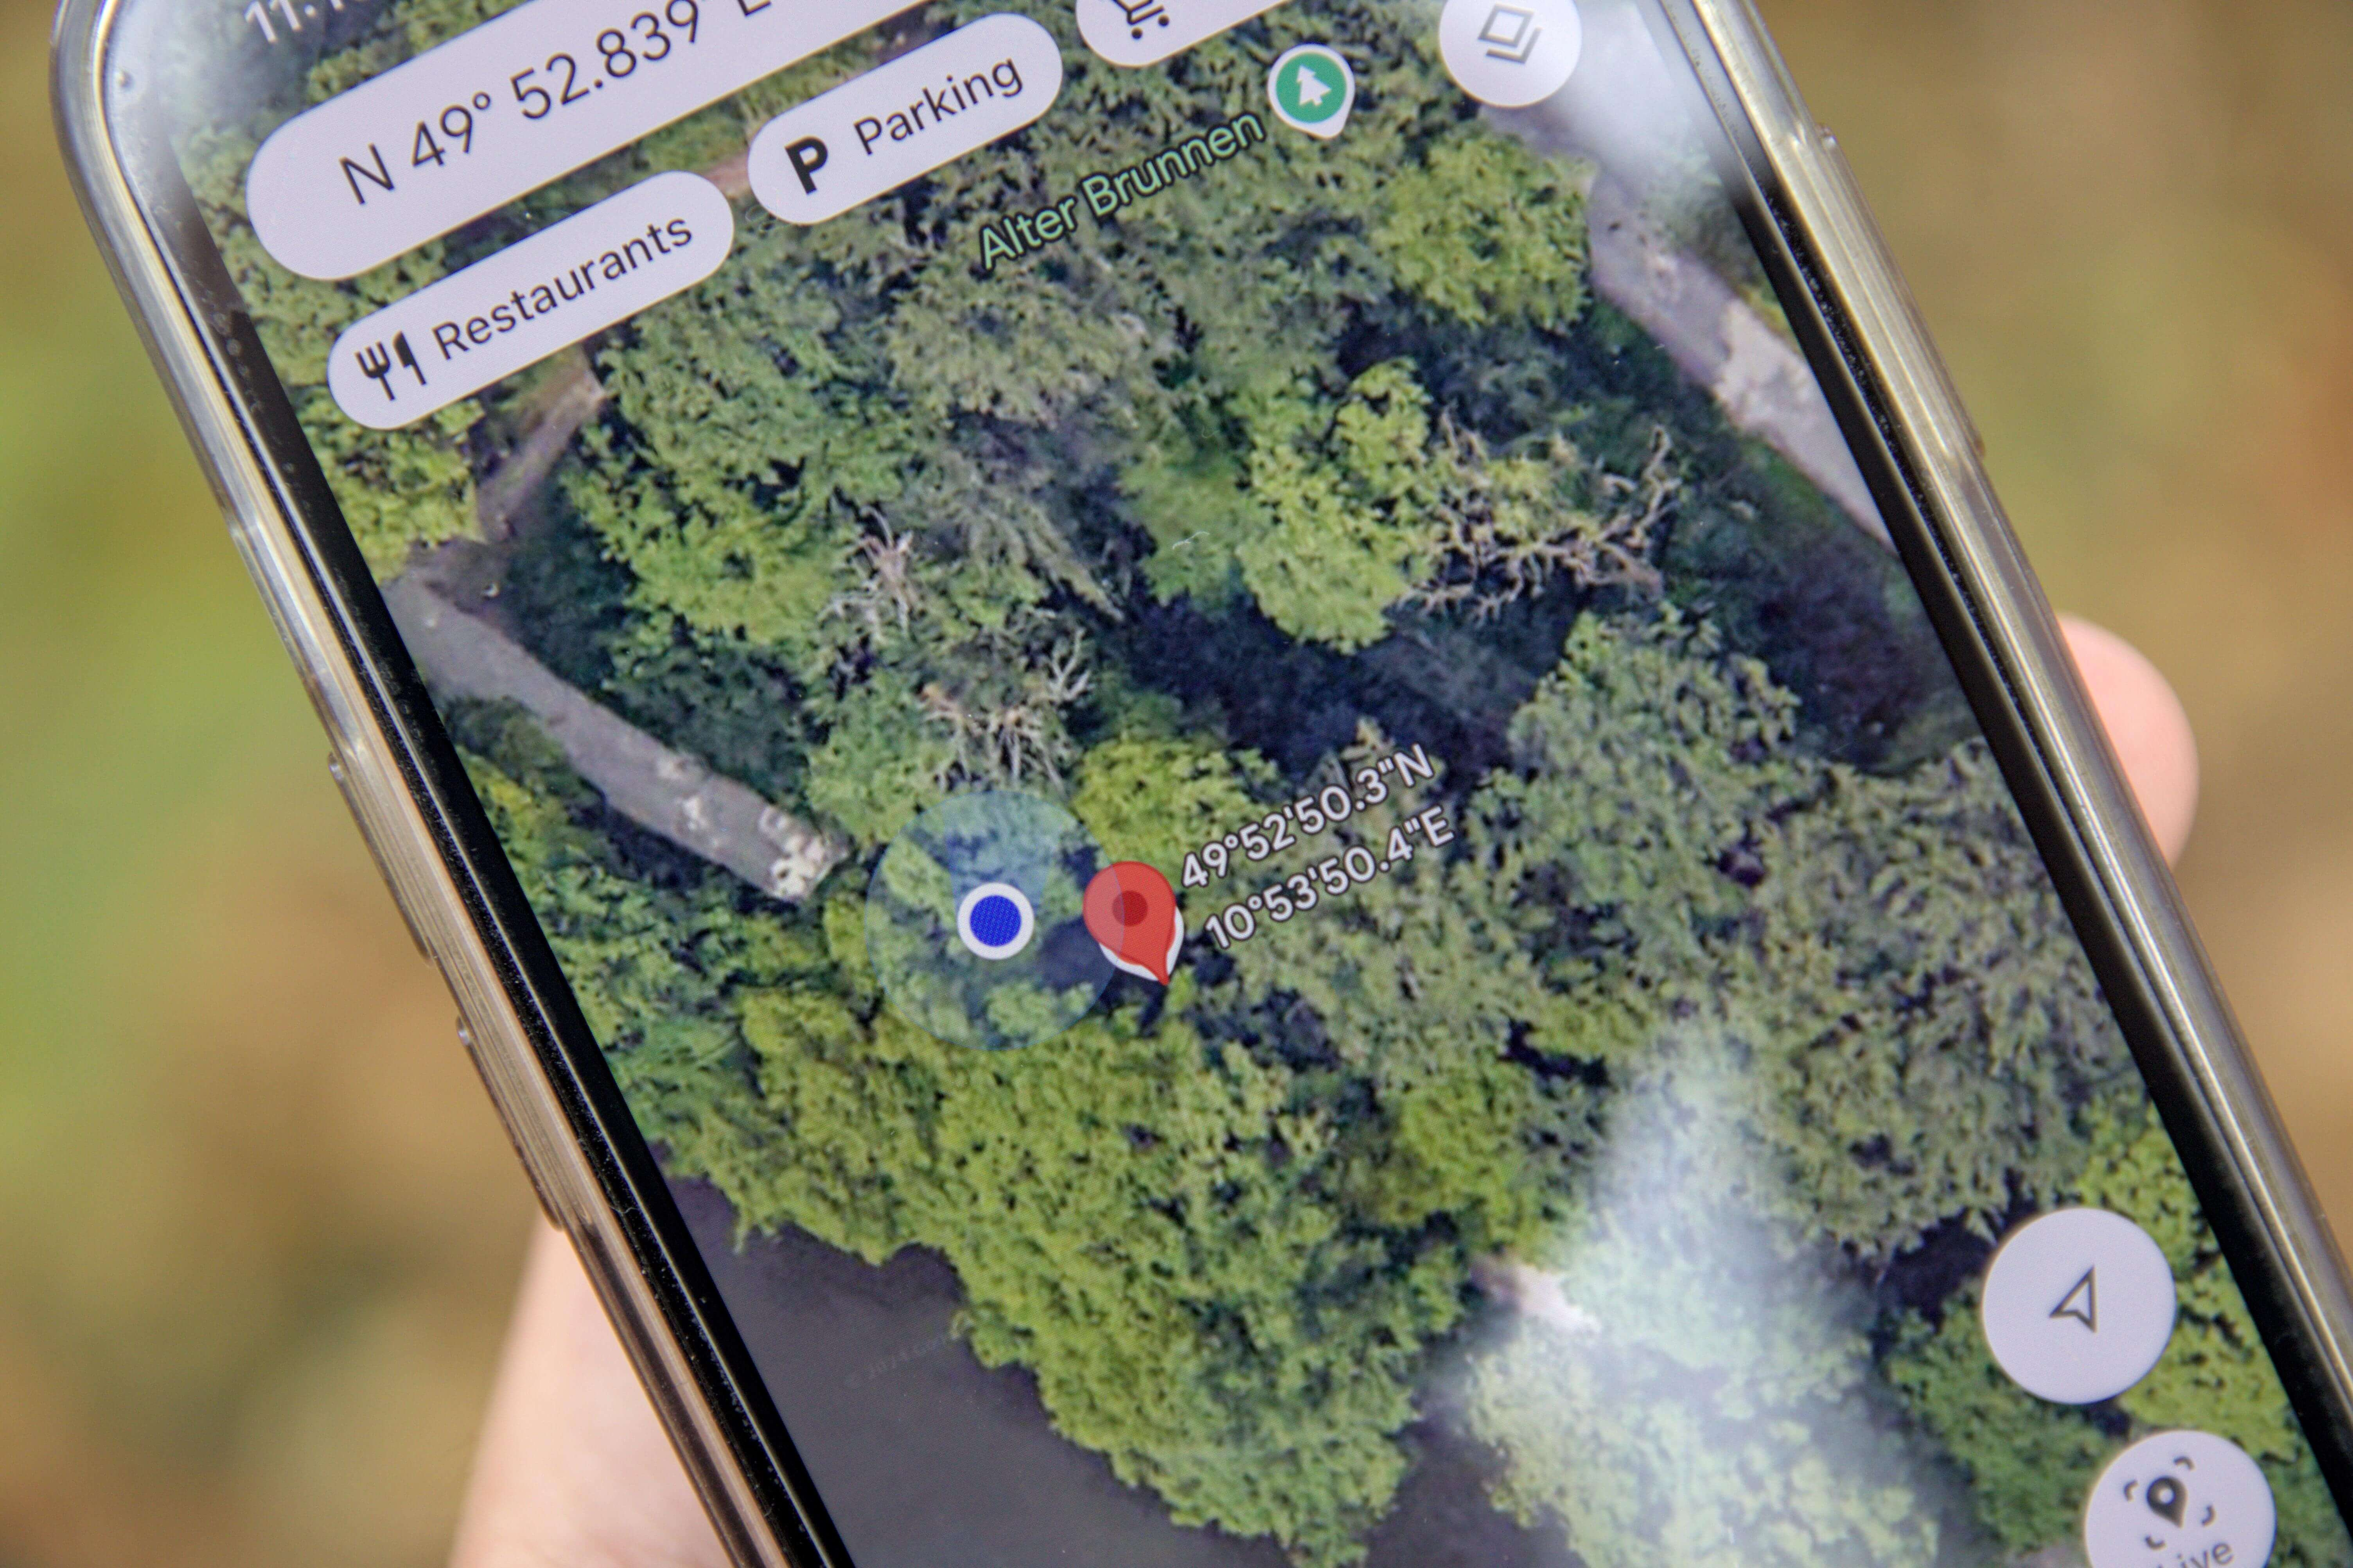
\includegraphics[width=.95\linewidth]{figures/geocaching/second/IMG_3118.jpg}
    \end{minipage}
    \caption{Alternativroute zum zweiten Cache, am Ziel angekommen.}
    \label{second-cache-weg}
\end{figure}

\begin{figure}[h]
    \centering
    \begin{minipage}{.6\textwidth}
        \centering
        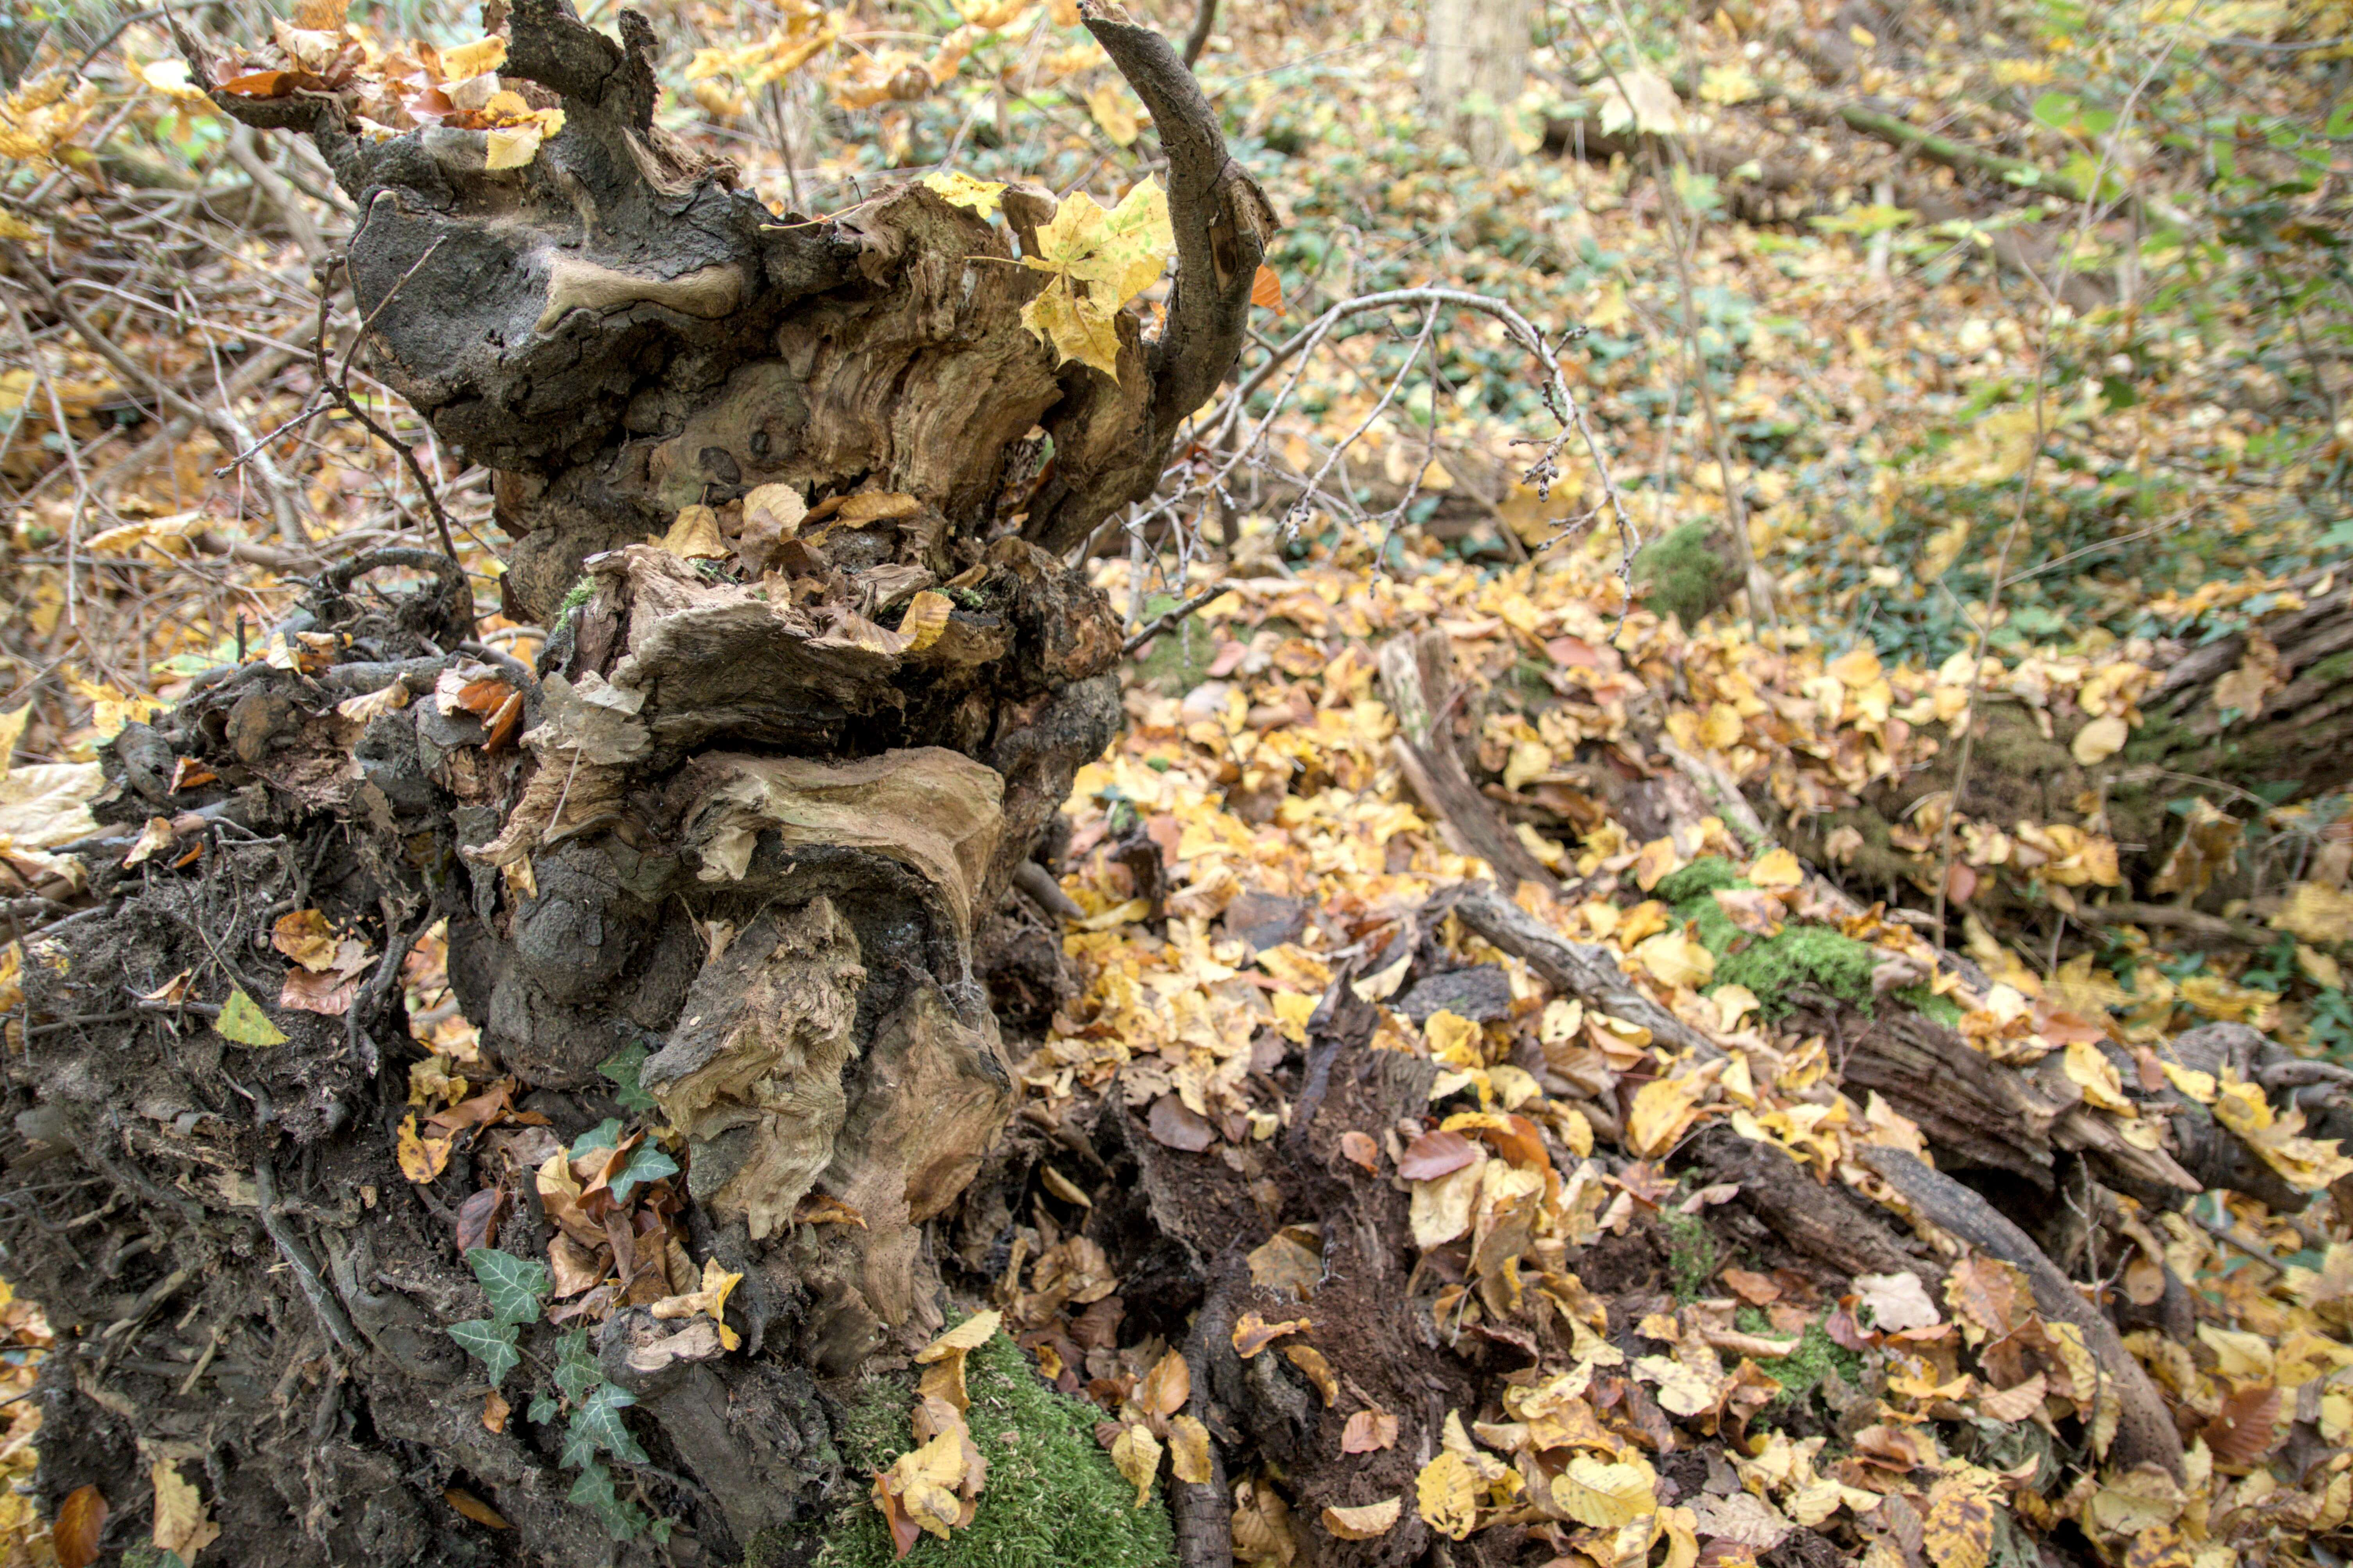
\includegraphics[width=\linewidth]{figures/geocaching/second/IMG_3109.jpg}
    \end{minipage}%
    \begin{minipage}{.4\textwidth}
        \centering
        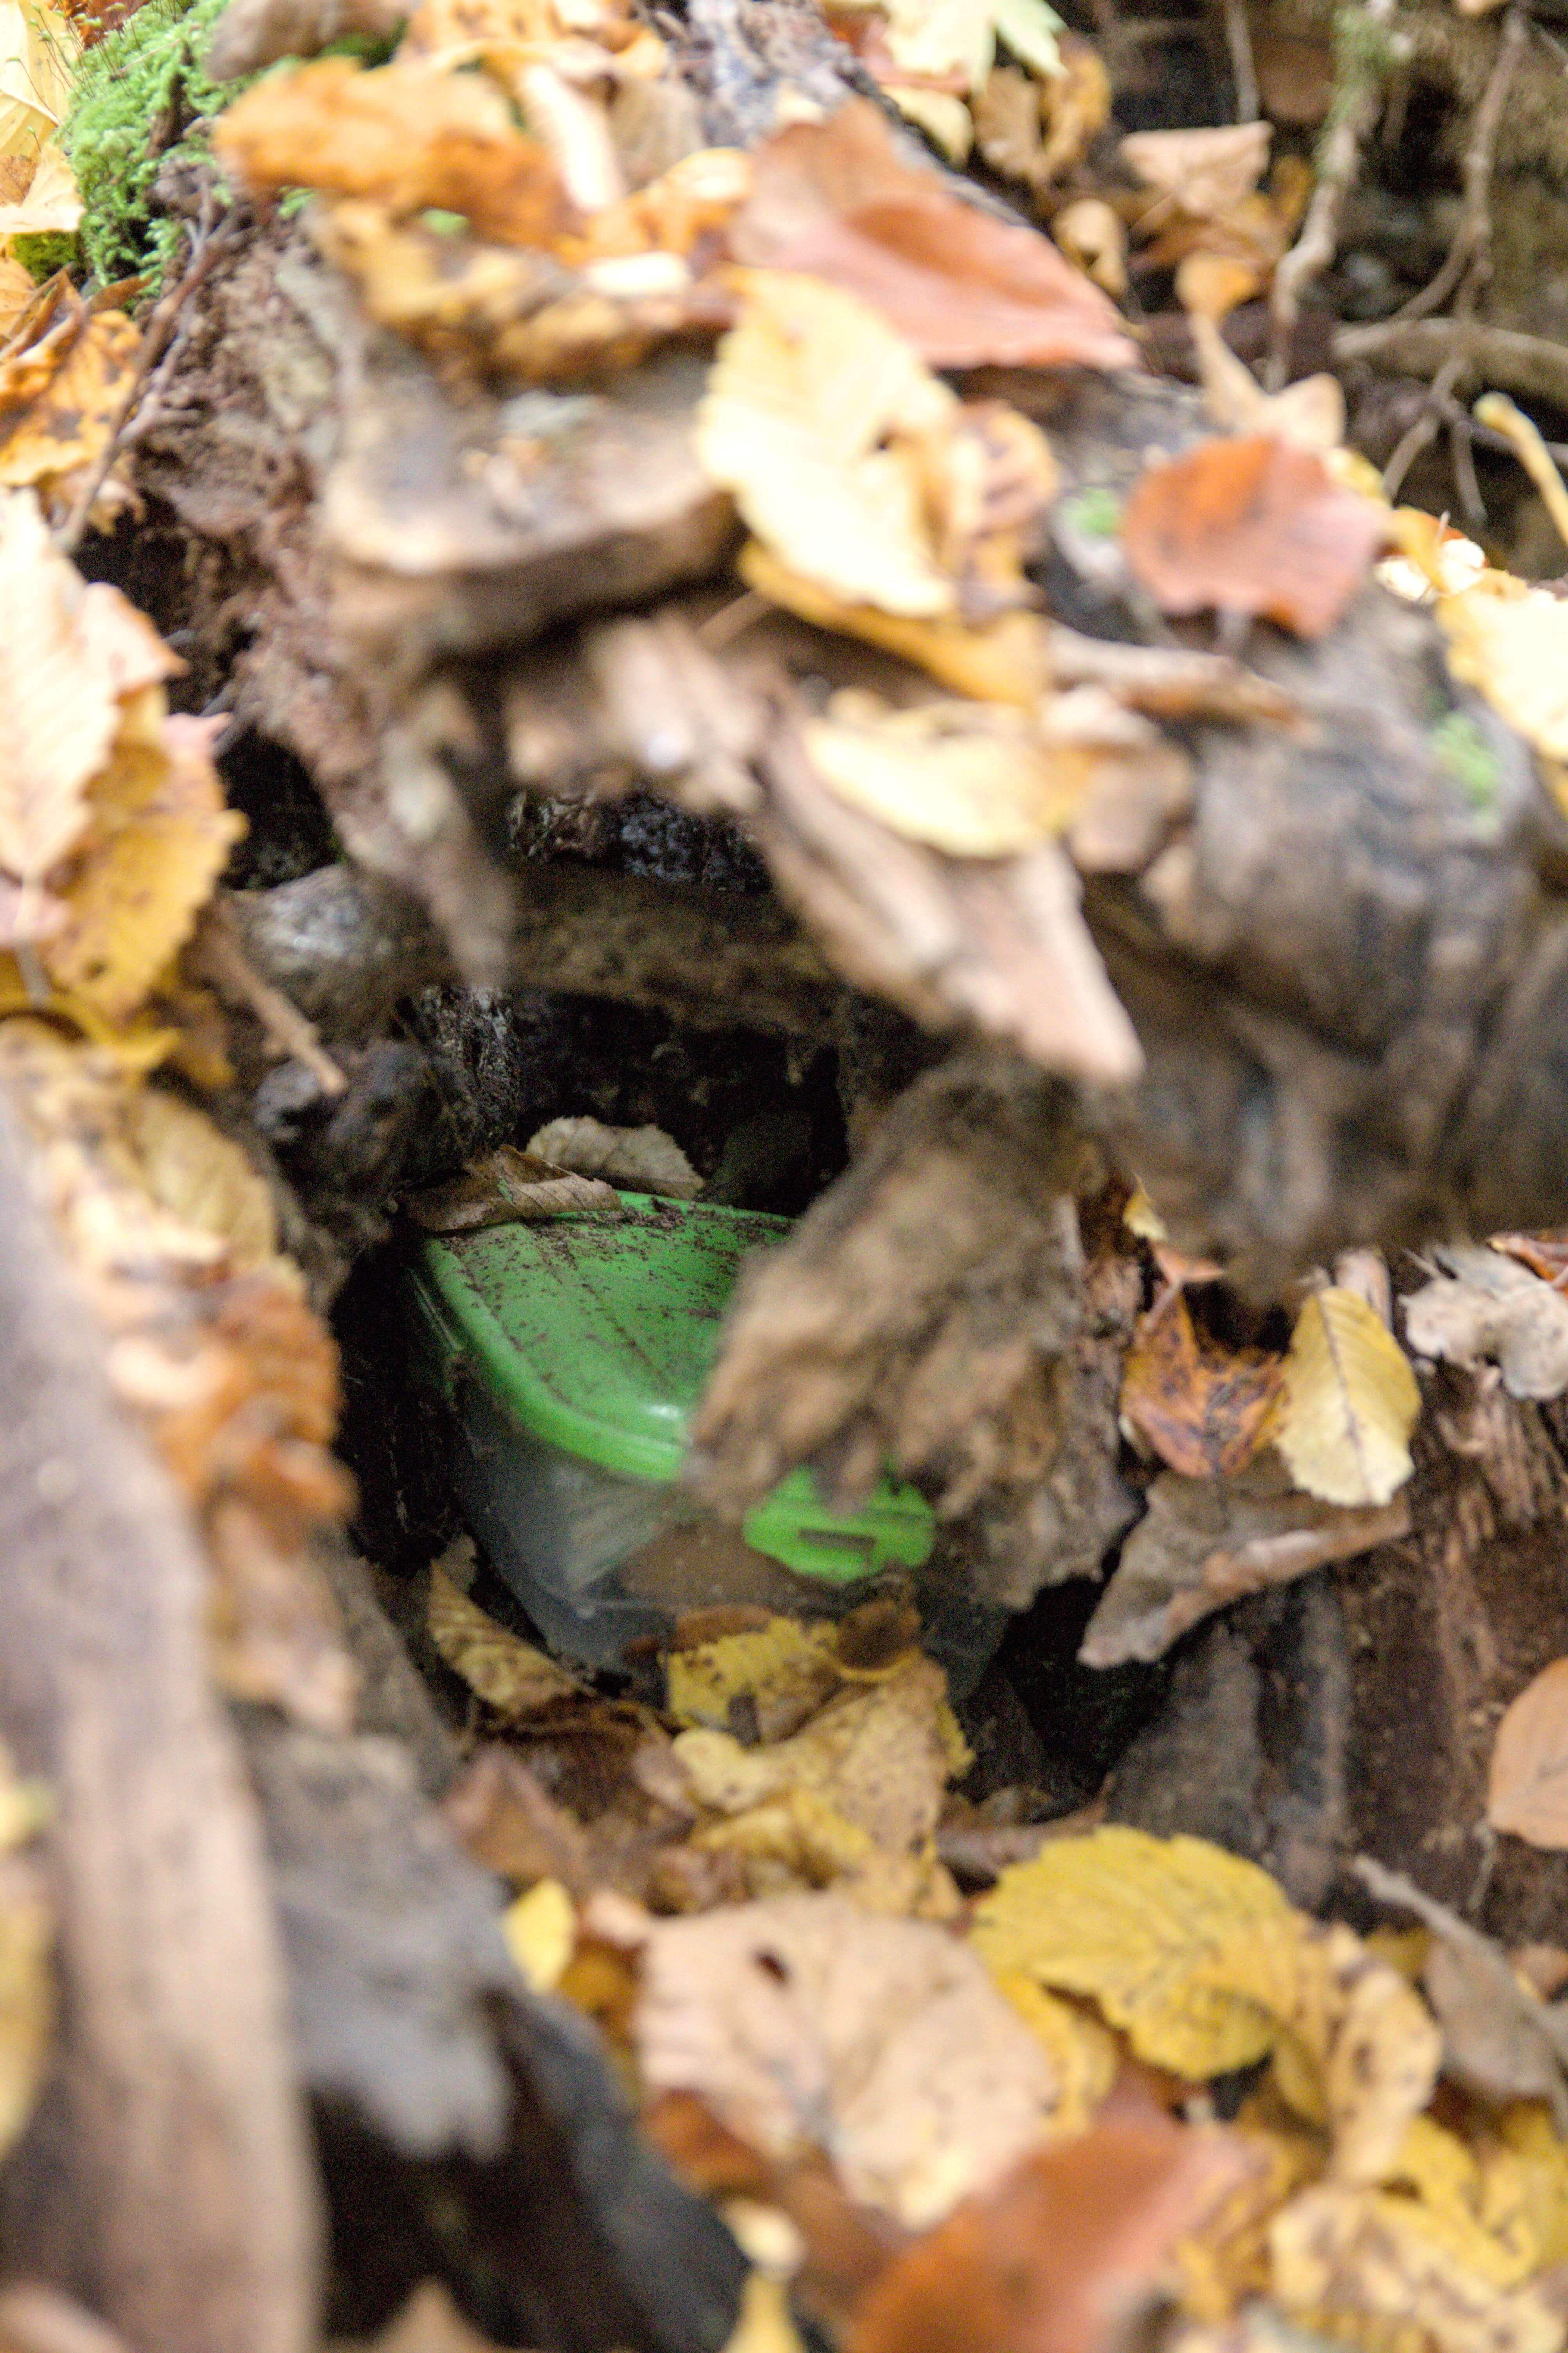
\includegraphics[width=.7\linewidth]{figures/geocaching/second/IMG_3112.jpg}
    \end{minipage}
    \caption{Das Versteck des zweiten Caches.}
    \label{second-cache-versteck}
\end{figure}

\begin{figure}[h]
    \centering
    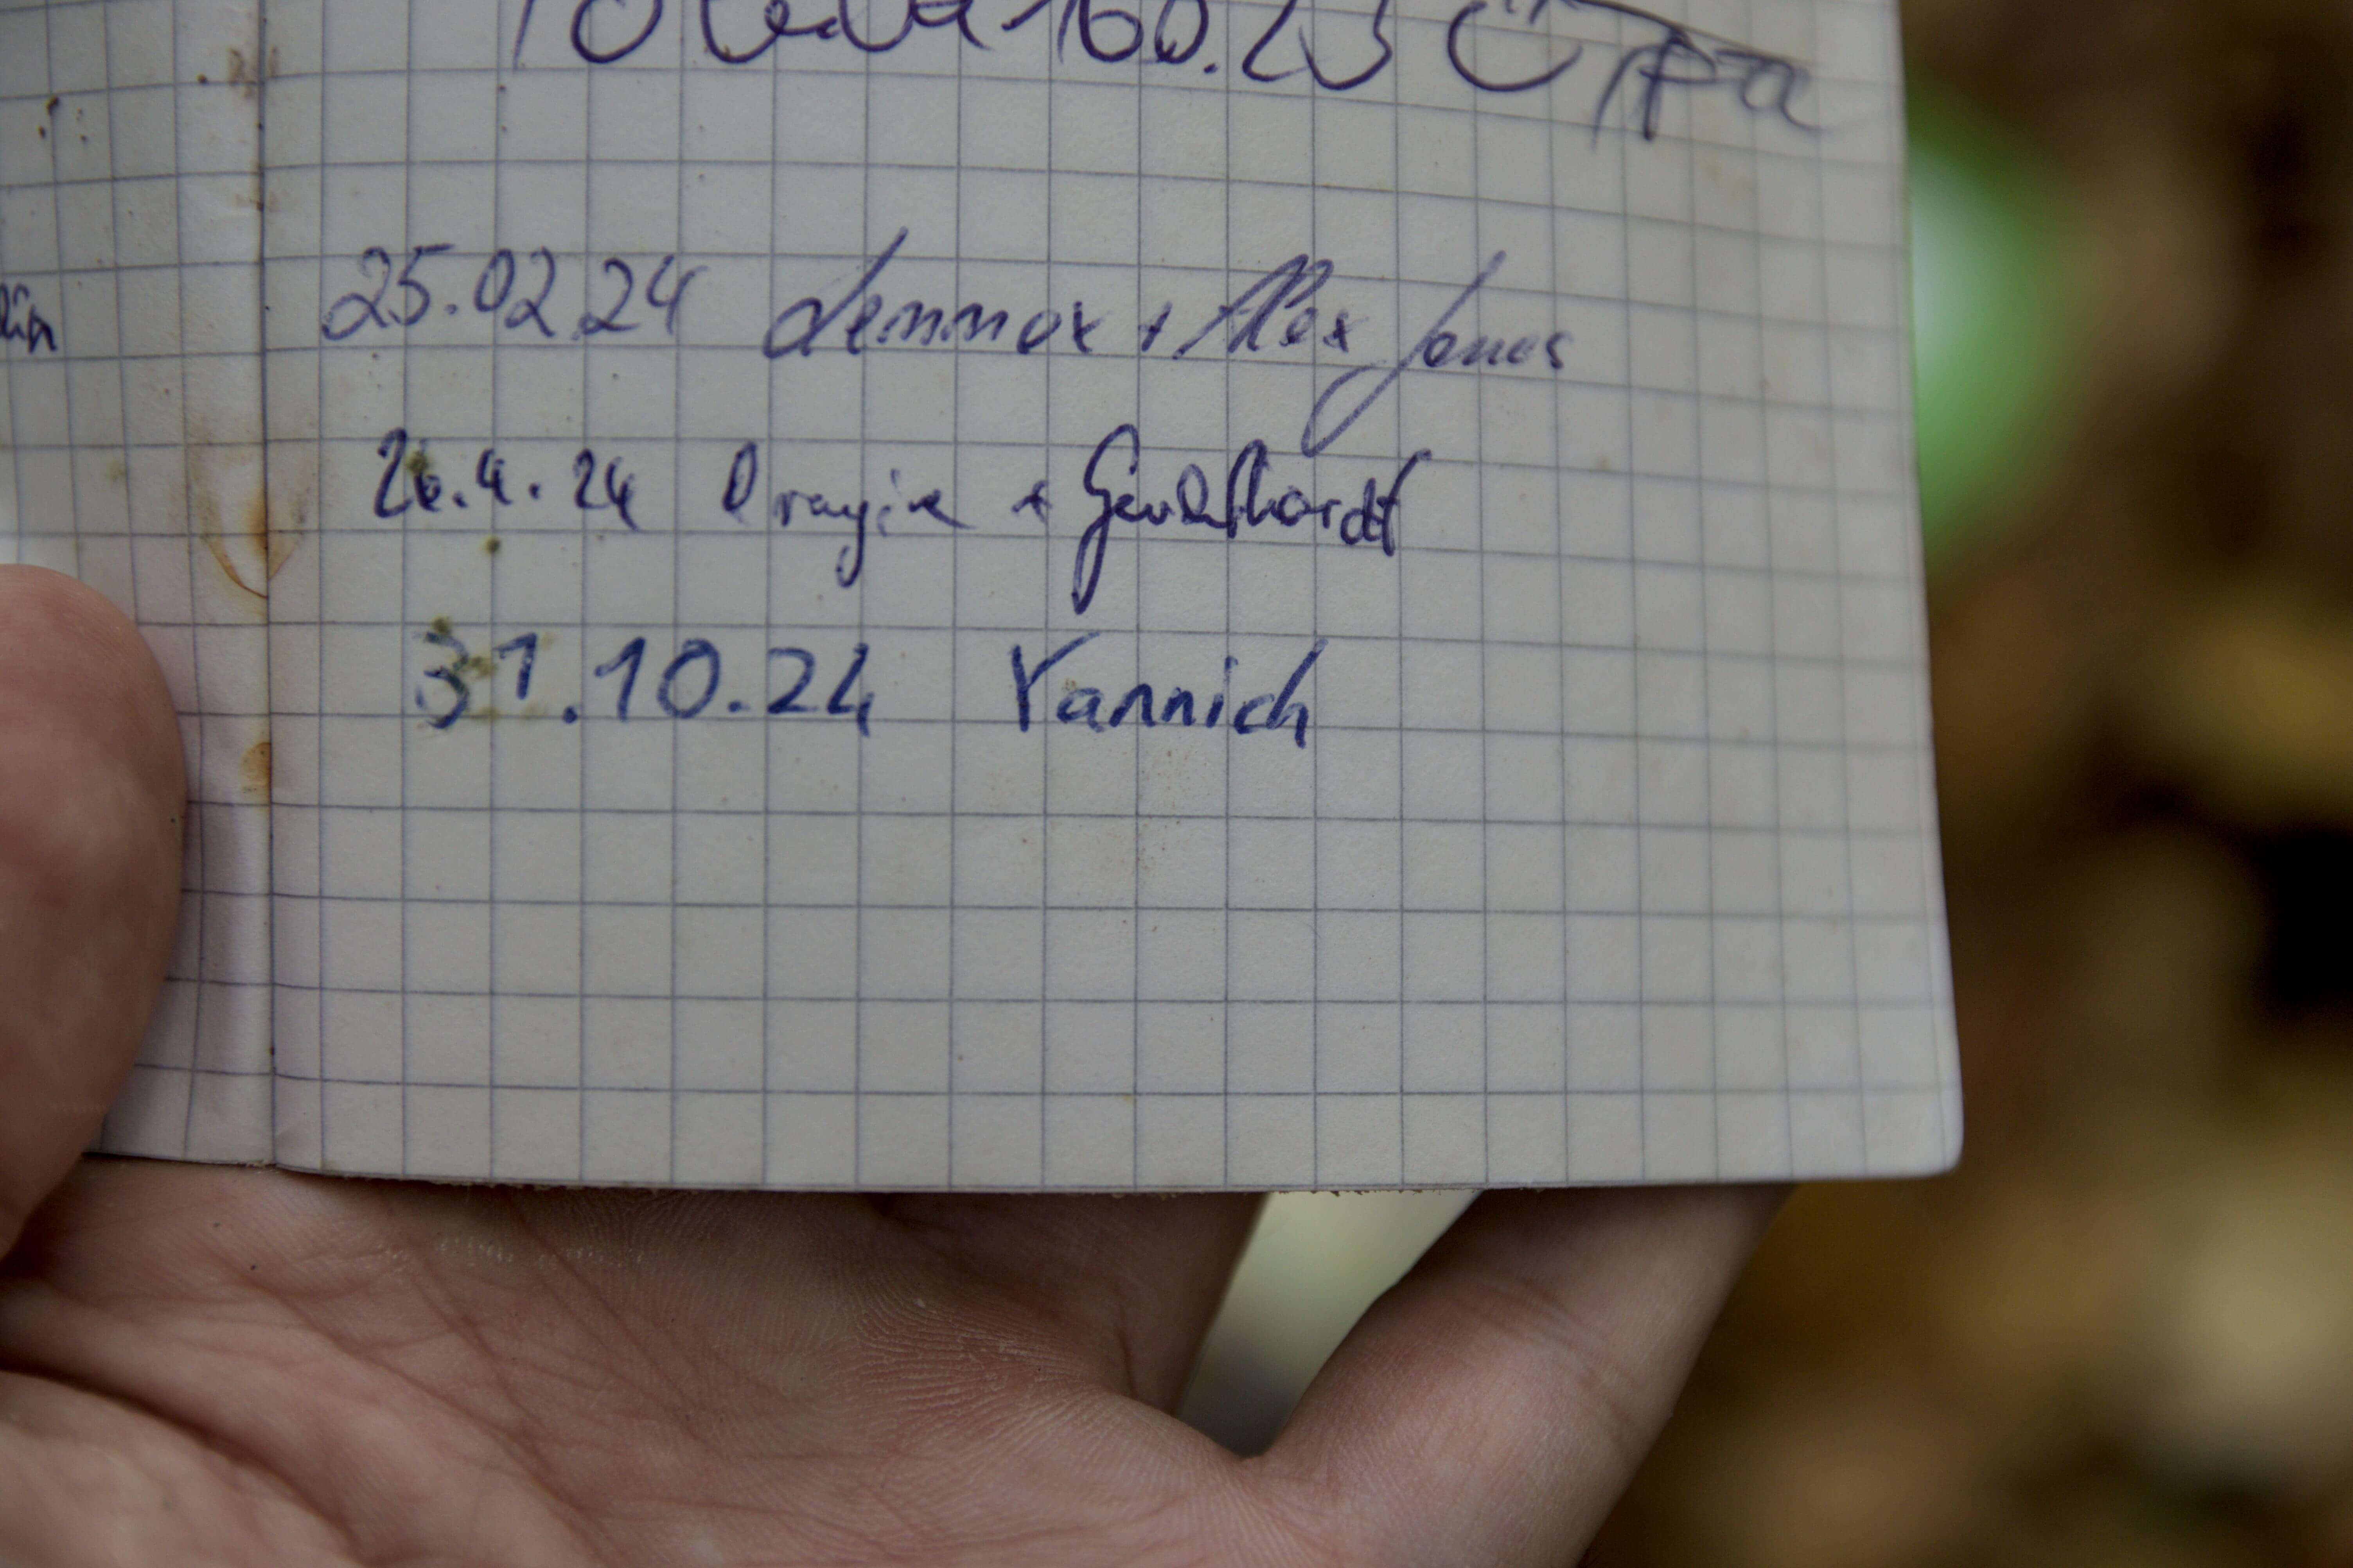
\includegraphics[width=.7\linewidth]{figures/geocaching/second/IMG_3113.jpg}
    \caption{Eintrag ins Logbuch.}
    \label{second-cache-log}
\end{figure}